\documentclass[conference]{IEEEtran}
\IEEEoverridecommandlockouts
% The preceding line is only needed to identify funding in the first footnote. If that is unneeded, please comment it out.
\usepackage{cite}
\usepackage{amsmath,amssymb,amsfonts}
\usepackage{algorithmic}
\usepackage{graphicx}
\usepackage[labelformat=parens, labelsep=space]{subcaption}

\usepackage{textcomp}
\usepackage[table, xcdraw]{xcolor} % The cell in the table can be highlighted
\usepackage{booktabs} % Use book tab style for all tables
\usepackage{lettrine} % Capticalize the first letter in the paper

% Equalize the colums of last page
\usepackage{flushend}

% Change label separator for figures and tables
\captionsetup[figure]{labelsep=period}
\captionsetup[table]{labelsep=period, font={scriptsize, sc}}


% Change index term to keywords
\renewcommand\IEEEkeywordsname{Keywords}

% Fix error when there is no bib item.
\def\BibTeX{{\rm B\kern-.05em{\sc i\kern-.025em b}\kern-.08em
    T\kern-.1667em\lower.7ex\hbox{E}\kern-.125emX}}

\makeatletter
\def\endthebibliography{%
  \def\@noitemerr{\@latex@warning{Empty `thebibliography' environment}}%
  \endlist
}

% Add a horizontal line for footnotes(thanks)
\def\footnoterule{\relax%
  \kern-5pt
  \hbox to \columnwidth{\hfill\vrule width 1\columnwidth height 0.4pt\hfill}
  \kern4.6pt}
\makeatother

\graphicspath{{figures/}}
\newtheorem{definition}{Definition}


\begin{document}
\title{Multi-modal Multi-objective Optimization: Problem Analysis and Case Studies
}
\author{\IEEEauthorblockN{Yiming Peng, Hisao Ishibuchi and Ke Shang}
\IEEEauthorblockA{Shenzhen Key Laboratory of Computational Intelligence,}
\IEEEauthorblockA{University Key Laboratory of Evolving Intelligent Systems of Guangdong Province,}
\IEEEauthorblockA{Department of Computer Science and Engineering, Southern University of Science and Technology (SUSTech), Shenzhen, China}
\IEEEauthorblockA{11510035@mail.sustech.edu.cn, hisao@sustech.edu.cn, kshang@foxmail.com}
\thanks{Corresponding Author: Hisao Ishibuchi (hisao@sustech.edu.cn)}
}

\maketitle

\begin{abstract}
In many real-world applications, multi-objective optimization problems may have more than one Pareto sets. The goal of multi-modal multi-objective optimization is to find all Pareto sets in the decision space. As a relatively new research area, difficulties in solving multi-modal multi-objective optimization problems have not been carefully analyzed in the literature. In this paper, first we point out that standard evolutionary multi-objective algorithms show difficulties when solving multi-modal multi-objective optimization problems. Next, using the concept of genetic drift, we clearly explain the decrease of diversity in the decision space during the evolutionary process. Then, we report performance evaluation results of state-of-the-art evolutionary multi-modal multi-objective algorithms using scalable test problems.
\end{abstract}

\bigskip %% Add a new line between abstract and keywords

\begin{IEEEkeywords}
\textit{Multi-modal multi-objective optimization; genetic drift; evolutionary algorithms}
\end{IEEEkeywords}

\section{Introduction}
Many real-world optimization problems require to optimize more than one objective functions which usually cannot be optimized simultaneously. In many cases, the fitness improvement in one objective function will cause fitness deterioration in other objectives. This kind of problems are usually referred to as Multi-objective Optimization Problems (MOPs). Multi-objective Evolutionary Algorithms (MOEAs) are designed for solving MOPs. Usually, MOEAs only consider the diversity of a solution set in the objective space. The diversity in the decision space has not gained much attention. However, in some cases, the diversity in the decision space is also very important, especially for Multi-modal Multi-objective Optimization Problems (MMOPs). An MMOP is a special type of an MOP which has more than one Pareto sets (PS) corresponding to the same PF. Many real-world optimization problems such as multi-objective knapsack problems \cite{jaszkiewicz2002performance} and game map generation problems \cite{togelius2010towards} have such property. An MMOP requires an optimizer to obtain a solution set that covers all Pareto sets. In engineering, some solutions are hard to implement due to physical limitations. In this case, obtaining multiple Pareto sets can help the decision maker to select an alternative solution with equivalent quality in the objective space. Besides, the knowledge about multiple Pareto sets may be helpful to better understand the structure of the optimization problem\cite{deb2001multi}. Evolutionary algorithms designed for solving MMOPs are named as Multi-modal Multi-objective Evolutionary Algorithms (MMEAs).

As pointed out in \cite{tanabe2019review} \cite{liang2016multimodal}, standard MOEAs do not perform well on MMOPs because they can obtain only a part of multiple Pareto sets in many cases. In this paper, first we confirm this through a series of computational experiments. Next, we explain why standard MOEAs do not work well on MMOPs. We illustrate that explicit mechanisms for maintaining the diversity of solutions in the decision space are necessary in order to handle MMOPs. This means that MMEAs should be able to preserve the diversity of solutions in both the decision and objective spaces. Since 2005, MMOPs have drawn attention of researchers in the MOEA community. Some new MMEAs were specially designed for MMOPs. Other MMEAs were proposed as modified versions of existing MOEAs. In this paper, several popular MMEAs are tested to examine their scalability in terms of the number of decision variables. We also compare the search ability of MMEAs to standard MOEAs.

The structure of this paper is as follows. In section \ref{Multi-modal Multi-objective Optimization}, we give the formal definition of MMOPs. We also explain diversity maintenance techniques in existing MMEAs and their characteristics. Section \ref{Difficulties Analysis} is devoted to analyze the difficulties in solving MMOPs. Then a series of computational experiments are conducted in section \ref{Experimental Studies}. Finally, this paper is concluded in section \ref{Conclusion}.
\section{Multi-modal Multi-objective Optimization}
\label{Multi-modal Multi-objective Optimization}
\subsection{Formal definition}
The formal definition of MMOPs can be described as follows\cite{tanabe2019review}:

\begin{definition}
\label{def: equivalent solution}
Solutions $\boldsymbol{x_1}$ and  $\boldsymbol{x_2}$ are equivalent  iff $||\boldsymbol{f}(\boldsymbol{x_1}) - \boldsymbol{f}(\boldsymbol{x_2})|| \leq \delta$ .
\end{definition}

\begin{definition}
MMOP is a kind of MOP that aims to find all solutions that are equivalent to Pareto optimal solutions. 
\end{definition}


In \textit{Definition} \ref{def: equivalent solution}, $\delta$ is a non-negative number that represents the tolerance of similarity of solutions given by the decision maker. If $\delta = 0$, the decision maker only accepts Pareto optimal solutions, and dominated solutions should be removed from the final solution set. A positive $\delta$ means that the decision maker can accept the sub-optimal solutions that are dominated by Pareto optimal solutions. Because it is difficult to accurately describe the relationship between the value of $\delta$ and the quality of the resulting solution set, we only consider the case of $\delta =0$ in our discussion. 

\subsection{Multi-polygon test problems}
There are several benchmark MMOPs used in the existing literature such as Omni-test \cite{deb2005omni} , SYM-PART \cite{rudolph2007capabilities} and multi-polygon\cite{ishibuchi2019salable} test problems. This paper uses multi-polygon test problems for analyzing the performance of MOEAs and MMEAs. This is because they have better flexibility than other test problems. A multi-polygon test problem is an MMOP based on the idea of distance minimization. For various version of multi-polygon problems, see \cite{fieldsend2019feature}, \cite{nojima2019constrained}.

As an example, let us consider four identical regular hexagons with radius $r$ in Fig. \ref{fig:Multi-Polygon Problem}. The distance $l$ between adjacent polygons should be larger than $4r$ (please refer to \cite{ishibuchi2019salable} for more details about the specification of $l$). With these settings, we can define a six-objective optimization problem as:

\begin{equation*}
\left\{
\begin{array}{c}{f_{1}(\boldsymbol{x})=\min \left\{d\left(\boldsymbol{x}, A_{1}\right), d\left(\boldsymbol{x}, B_{1}\right), d\left(\boldsymbol{x}, C_{1}\right), d\left(\boldsymbol{x}, D_{1}\right)\right\}} \\ \dots \\ {{f_{6}}(\boldsymbol{x})=\min \left\{d\left(\boldsymbol{x}, A_{6}\right), d\left(\boldsymbol{x}, B_{6}\right), d\left(\boldsymbol{x}, C_{6}\right), d\left(\boldsymbol{x}, D_{6}\right)\right\}}\end{array}
\right.
\end{equation*}
where $d(\boldsymbol{a} ,\boldsymbol{b})$ is the Euclidean distance between vectors $\boldsymbol{a}$ and $\boldsymbol{b}$ (i.e., between points $\boldsymbol{a}$ and $\boldsymbol{b}$). In this test problem, any point inside the four hexagons is Pareto optimal. Therefore, this test problem has four equivalent Pareto sets. Compared to other MMOPs which have fixed number of decision variables, the multi-polygon test problem is much more flexible. For multi-polygon test problem, the number of objectives, decision variables, equivalent Pareto sets and local Pareto sets can be arbitrary specified\cite{ishibuchi2019salable}.

\begin{figure}[t!]
	\centering
	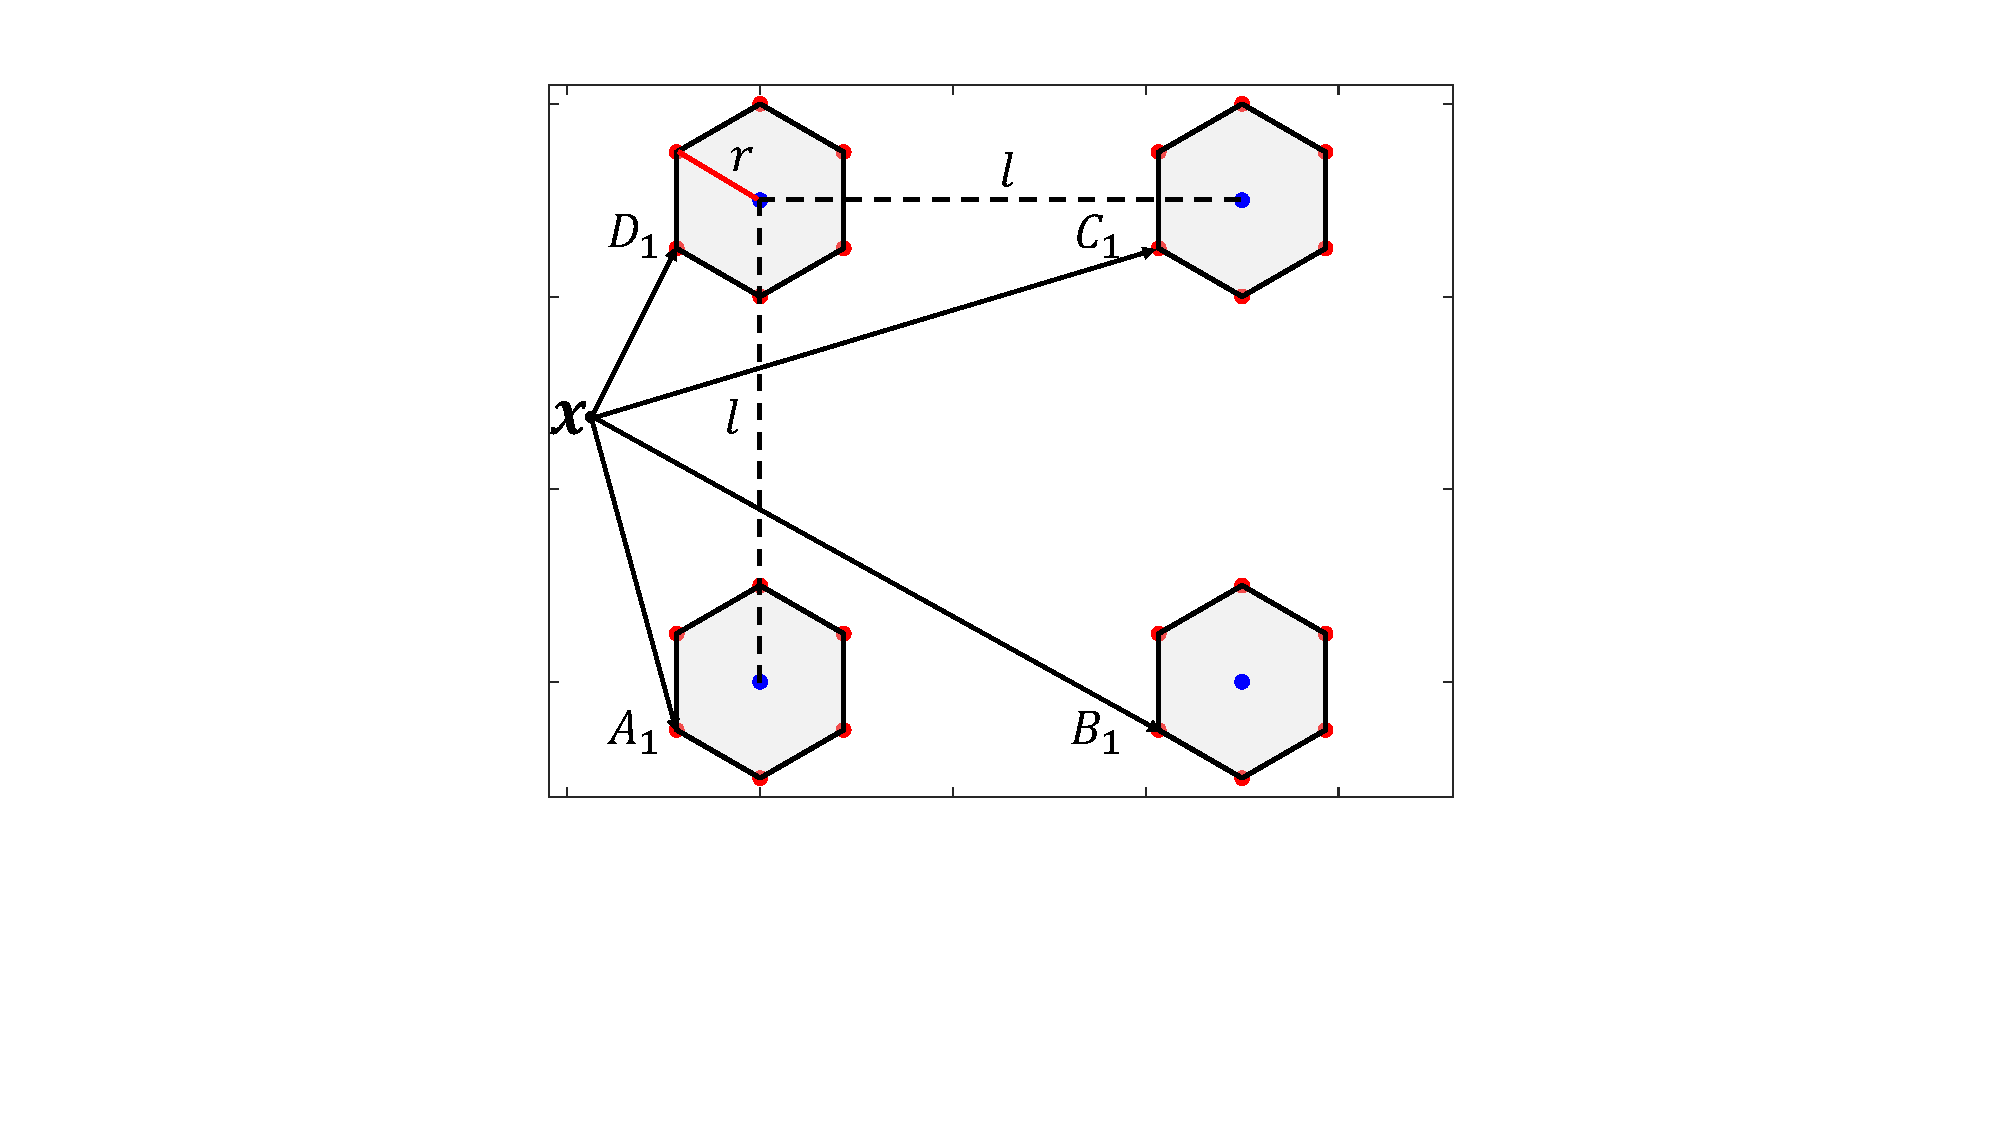
\includegraphics[width=.25\textwidth]{Section2/Problem}
	\caption{An example of multi-polygon test problem.}
	\label{fig:Multi-Polygon Problem}
\end{figure}

\subsection{Review of diversity maintenance techniques in MMEAs}
\label{Review of State-of-the-art Techniques}
In this section, we provide a short review of frequently used techniques to preserve the diversity of solutions in the decision space in MMEAs. As pointed out by Deb \cite{deb2001multi}, the key idea to solve MMOPs is to "divide" the entire population into several sub-populations and let each sub-population evolve independently. Here we list some commonly used approaches:
\subsubsection{Fitness Sharing Approach}
Fitness sharing was initially introduced in \cite{goldberg1987genetic} and widely used in MOEAs to maintain the diversity of the solutions in the objective space. The main idea of fitness sharing is to degrade the fitness of crowded solutions. In order to solve MMOPs, fitness sharing in both decision and objective spaces needs to be considered simultaneously. For example, DNEA\cite{liu2018double} uses the sum of two fitness sharing functions for the decision and objective spaces. Fitness sharing is hard to applied in real world applications because the sharing radius is problem dependent and hard to be specified.
\subsubsection{Crowding Distance Approach}
Crowding distance is often used as a second environmental selection criterion in Pareto-dominance based MOEAs such as NSGA-II\cite{deb2002fast} to ensure that obtained solutions are spread uniformly in the objective space. Several MMEAs such as Omni-optimizer\cite{deb2005omni} and MO\_Ring\_PSO\_SCD\cite{yue2017multiobjective} design special types of crowding distance that take both the decision and objective spaces into account.
\subsubsection{Restricted Environmental Selection Approach}
Performing the environmental selection in the whole population is harmful to the population diversity in the decision space, which will be explained in Section \ref{Difficulties Analysis}. One remedy is to restrict the environmental selection in part of the population. More specifically, a solution should compete with its neighborhood solutions in the decision space. The neighborhood relationship may either distance based or index based. For example, in MOEA/D-AD \cite{tanabe2018decomposition}, a solution $\boldsymbol{x}$ only competes with the closest $L$ solutions in the decision space.

\section{Difficulties in Solving MMOPs}
\label{Difficulties Analysis}
Although a number of studies on MMOPs have been published, difficulties in solving MMOPs are not analyzed in many studies. In this section, we analyze the difficulties of maintaining the diversity of the population in the decision space. Although our analysis is based on the multi-polygon test problems, discussion in this section can be generalized to other MMOPs. Now we analyze the difficulties in solving MMOPs from the following three aspects:

\subsection{Environmental selection}
\label{Impact of environmental selection}
In most MOEAs, the environmental selection acts on the whole population. This usually leads to the following consequences in MMOPs.
A relatively good solution eliminates some other dominated solutions even if they are far away in the decision space. As mentioned in \cite{liang2016multimodal}, in MMOPs, two solutions that are not close in the decision space can be very close or even overlapped in the objective space. Thus MOEAs remove solutions crowded in the objective space even if they are far away in the decision space. As a result, it is likely that equivalent (or slightly inferior) solutions will be eliminated. As Fig. \ref{fig: Environmental selection} shows, both a Pareto dominance-based mechanism and a crowding-based mechanism decrease the diversity of solutions in the decision space. 

\begin{figure}[t!]
	\centering
	\begin{subfigure}[b]{.3\textwidth}
		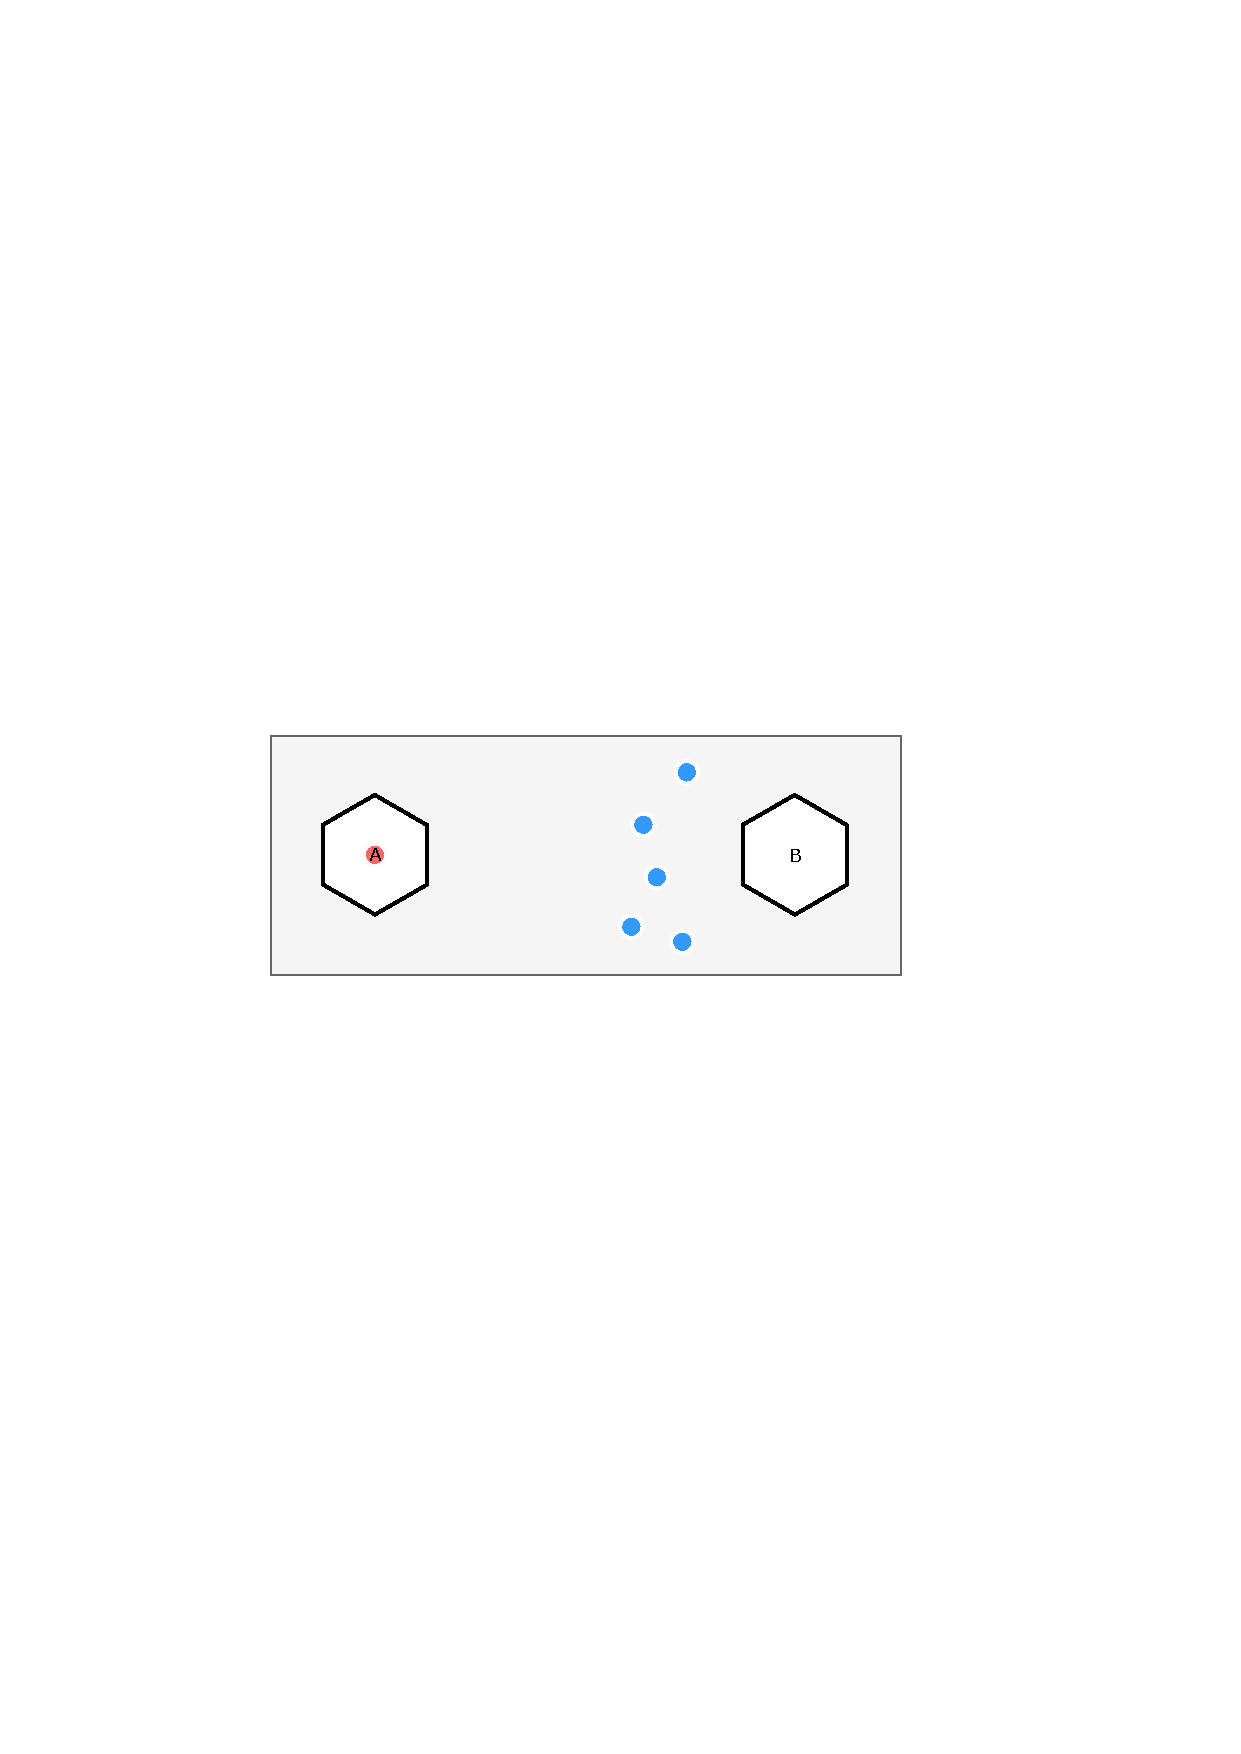
\includegraphics[width=\linewidth]{Section3/case1}
		\caption{Case 1: The blue solutions are dominated by the red one.}
	\end{subfigure}
	
	\begin{subfigure}[b]{.3\textwidth}
		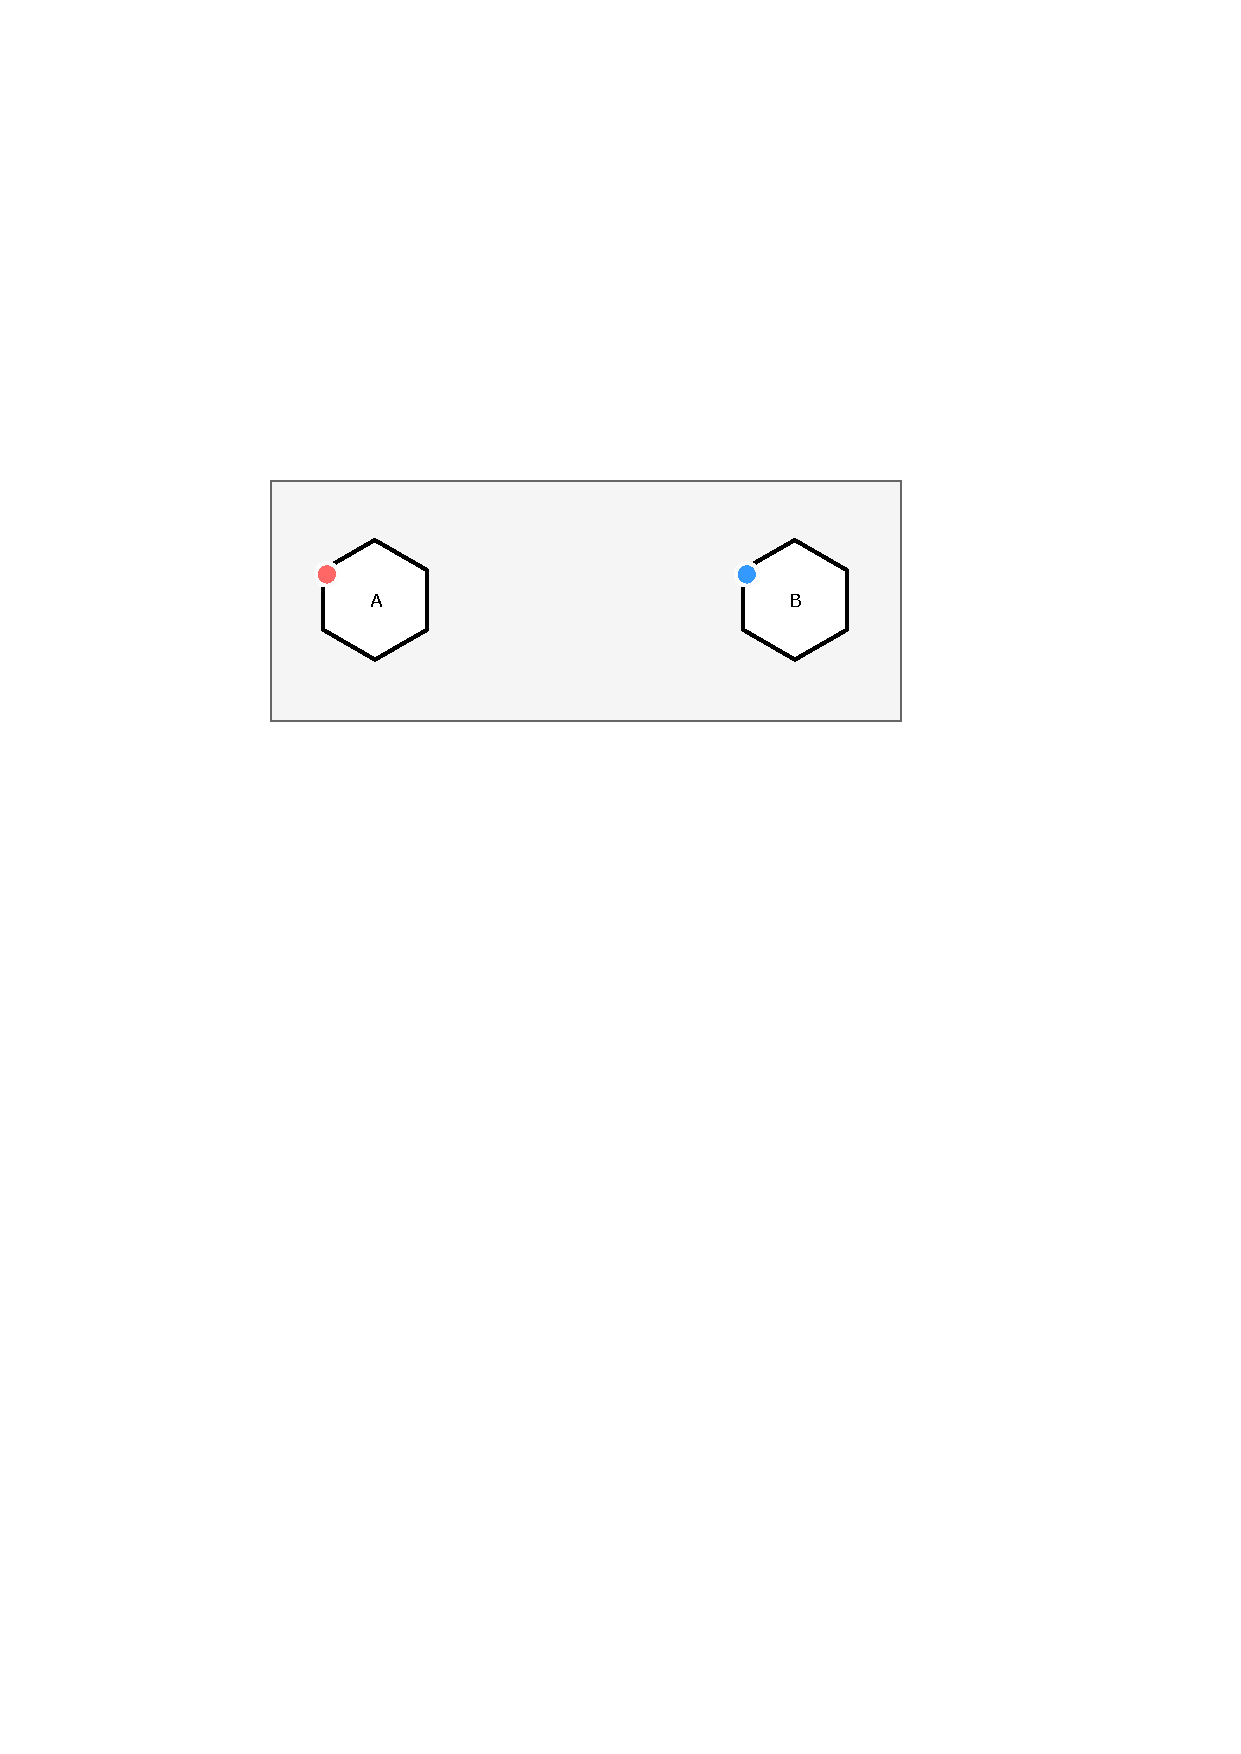
\includegraphics[width=\linewidth]{Section3/case2}
		\caption{Case 2: The two solutions are equivalent in the objective space.}
	\end{subfigure}
	\caption{The impact of environmental selection on the diversity of the population in the decision space. In (a), the red solution can survive. In (b), one of the two solutions can survive. }
	\label{fig: Environmental selection}
\end{figure}

\subsection{Genetic drift}
The decrease in the diversity of solutions in the decision space is also related to the concept of \textit{Genetic Drift}. Genetic drift is a phenomenon in which the frequency of alleles in a population declines due to random sampling errors \cite{muhlenbein1993predictive}. Fig. \ref{fig:Genetic drift demo} gives an example of genetic drift. At generation $t$, the population contains the same number of alleles $A$ and $a$. Let us assume that only random sampling is performed (no selection, mutation and crossover) from generation $t$ to $t+1$. Then the frequency of $A$ can become larger than $a$ in generation $t+1$ due to the random sampling error. After a number of generation updates based on random sampling, allele $A$ can become extinct.

\begin{figure}[t!]
	\centering
	\begin{subfigure}[b]{.24\textwidth}
		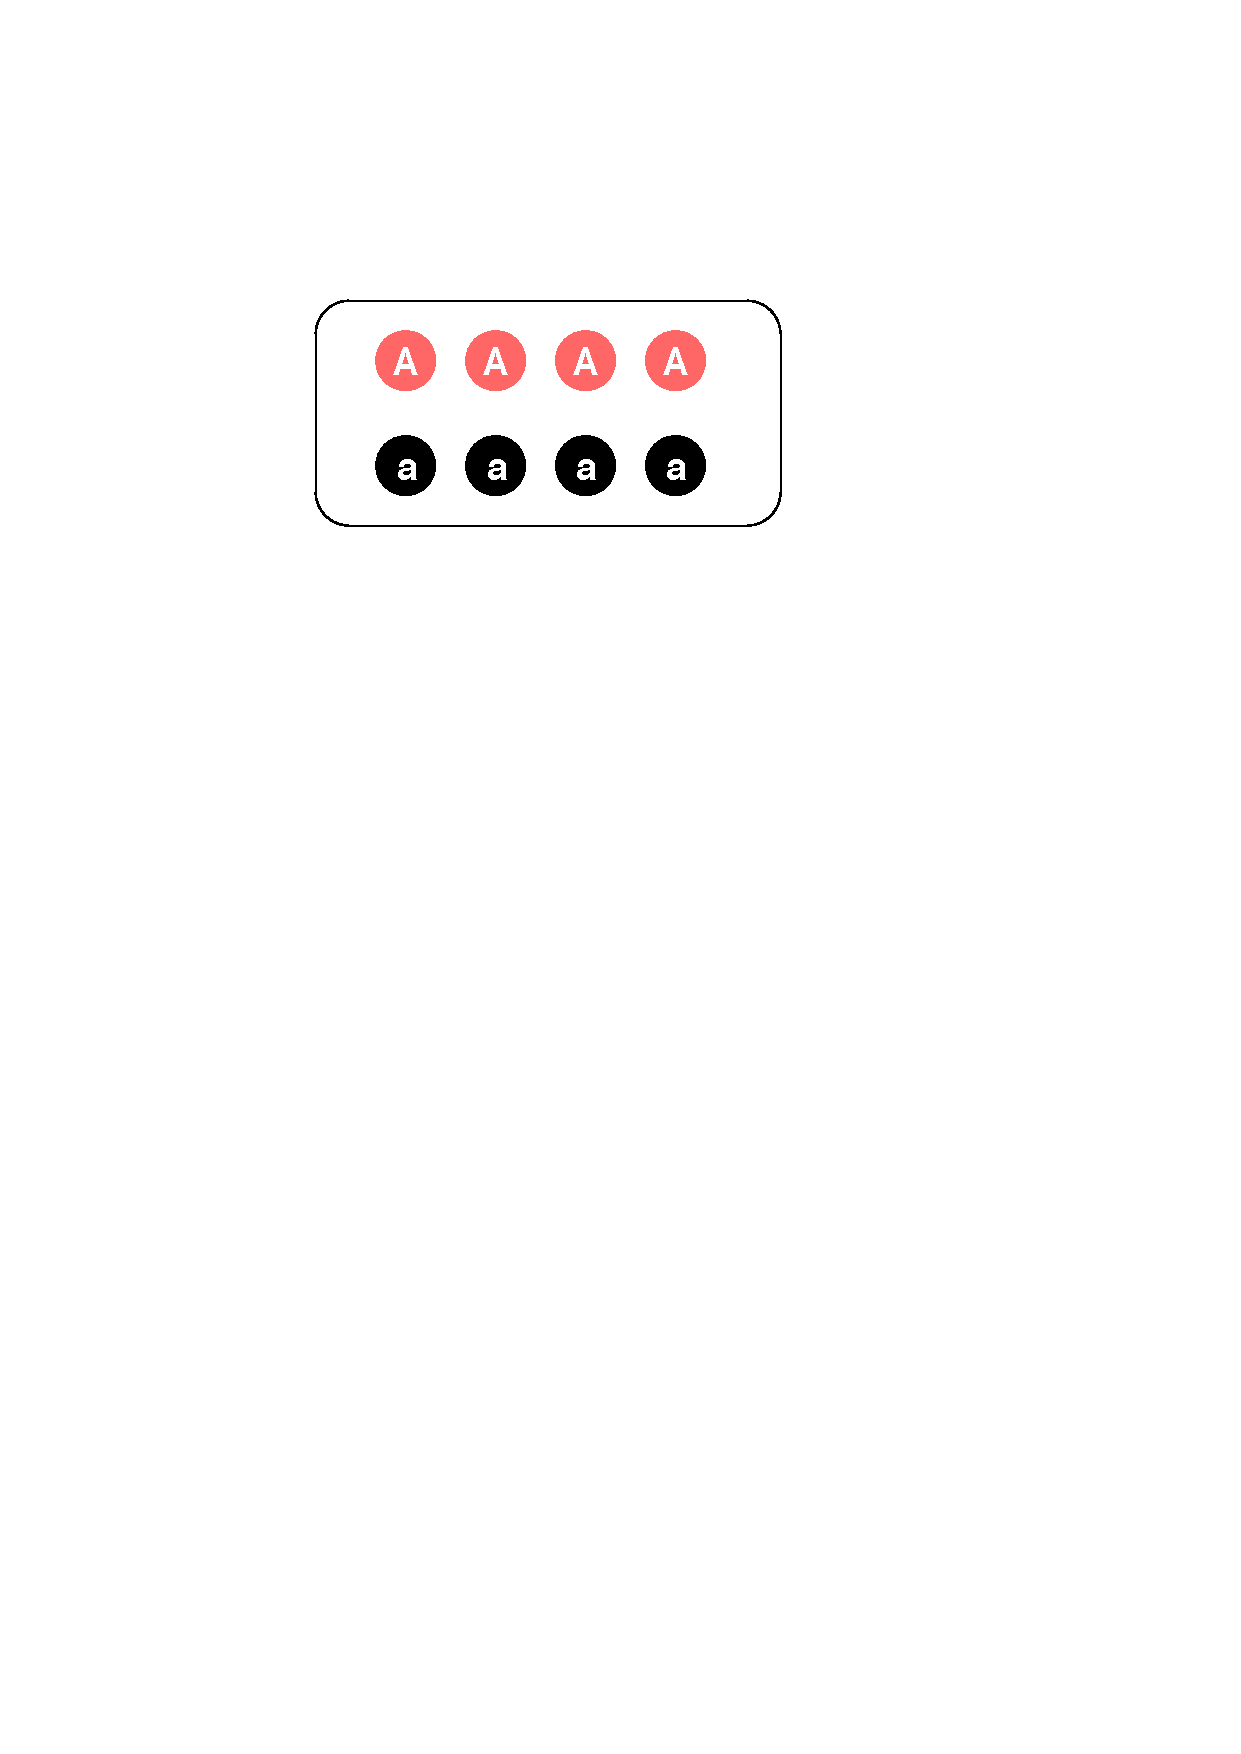
\includegraphics[width=\linewidth]{Section2/Generation_t}
		\caption{Generation $t$}
	\end{subfigure}
	\begin{subfigure}[b]{.24\textwidth}
		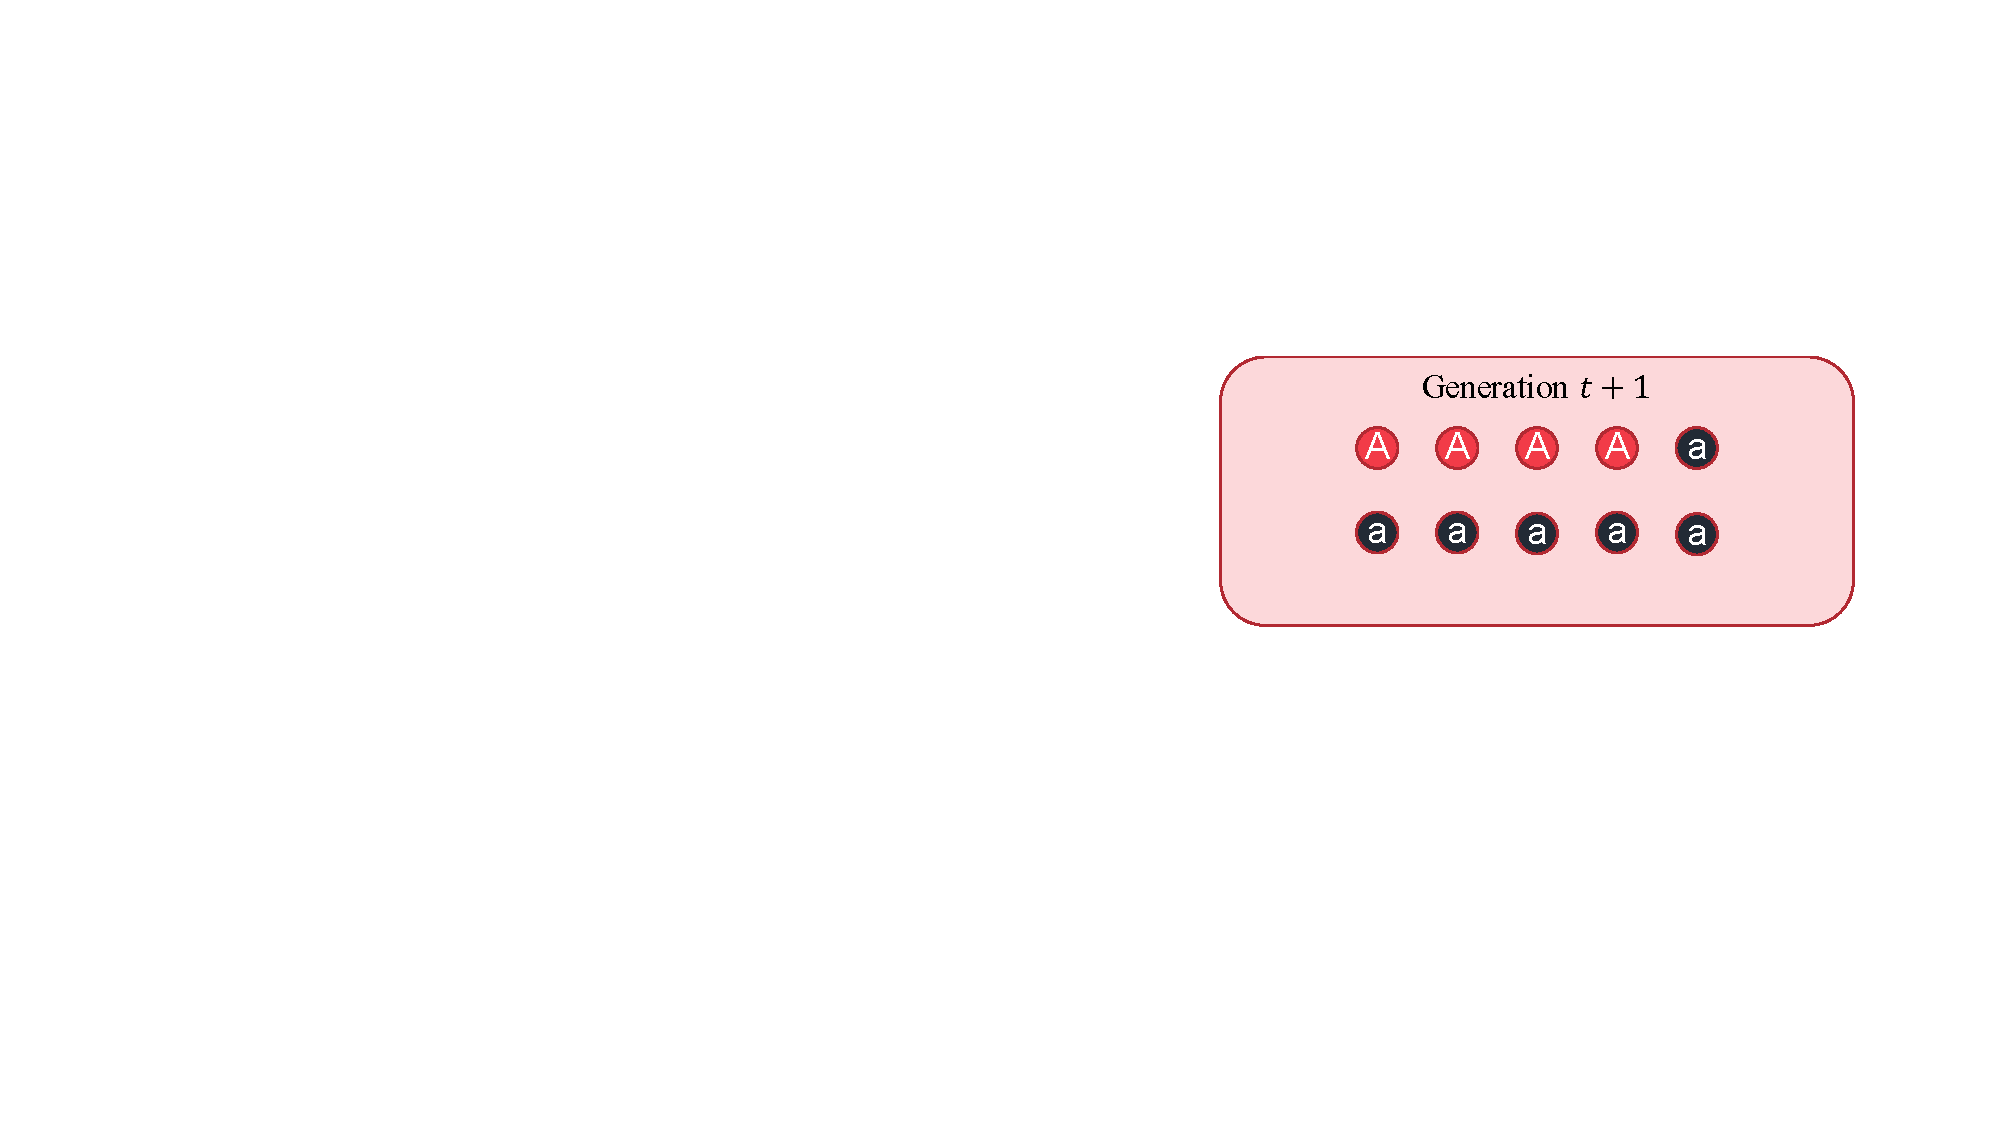
\includegraphics[width=\linewidth]{Section2/Generation_t1}
		\caption{Generation $t+1$}
	\end{subfigure}
	\caption{Demonstration of genetic drift}
	\label{fig:Genetic drift demo}
\end{figure}

Genetic drift tends to reduce the genetic variation of the population during the evolutionary process. Some alleles can disappear due to genetic drift as explained in Fig. \ref{fig:Genetic drift demo}. Asoh\cite{asoh1994mean} mathematically proved the following when only random selection is performed: only one of alleles in the population survives (this process is called convergence) as the iteration proceeds, and the mean convergence time varies in direct proportion with the population size. 

In Fig. \ref{fig: Alleles}, we divide the decision space of a multi-polygon problem into four parts. Since the four parts are mapped to exactly the same set in the objective space, they can be viewed as different alleles with the same fitness for simplicity of discussions. It is likely that three parts will disappear after a large number of generations.

Genetic drift can affect the distribution of the population in the decision space throughout the evolution process. In general, due to the existence of genetic drift, the diversity in the decision space will reduce. In section \ref{Experimental Studies}, we use computational experiments to study the effects of genetic drift on the search behavior of standard MOEAs on MMOPs.

\begin{figure}[t!]
    \centering
    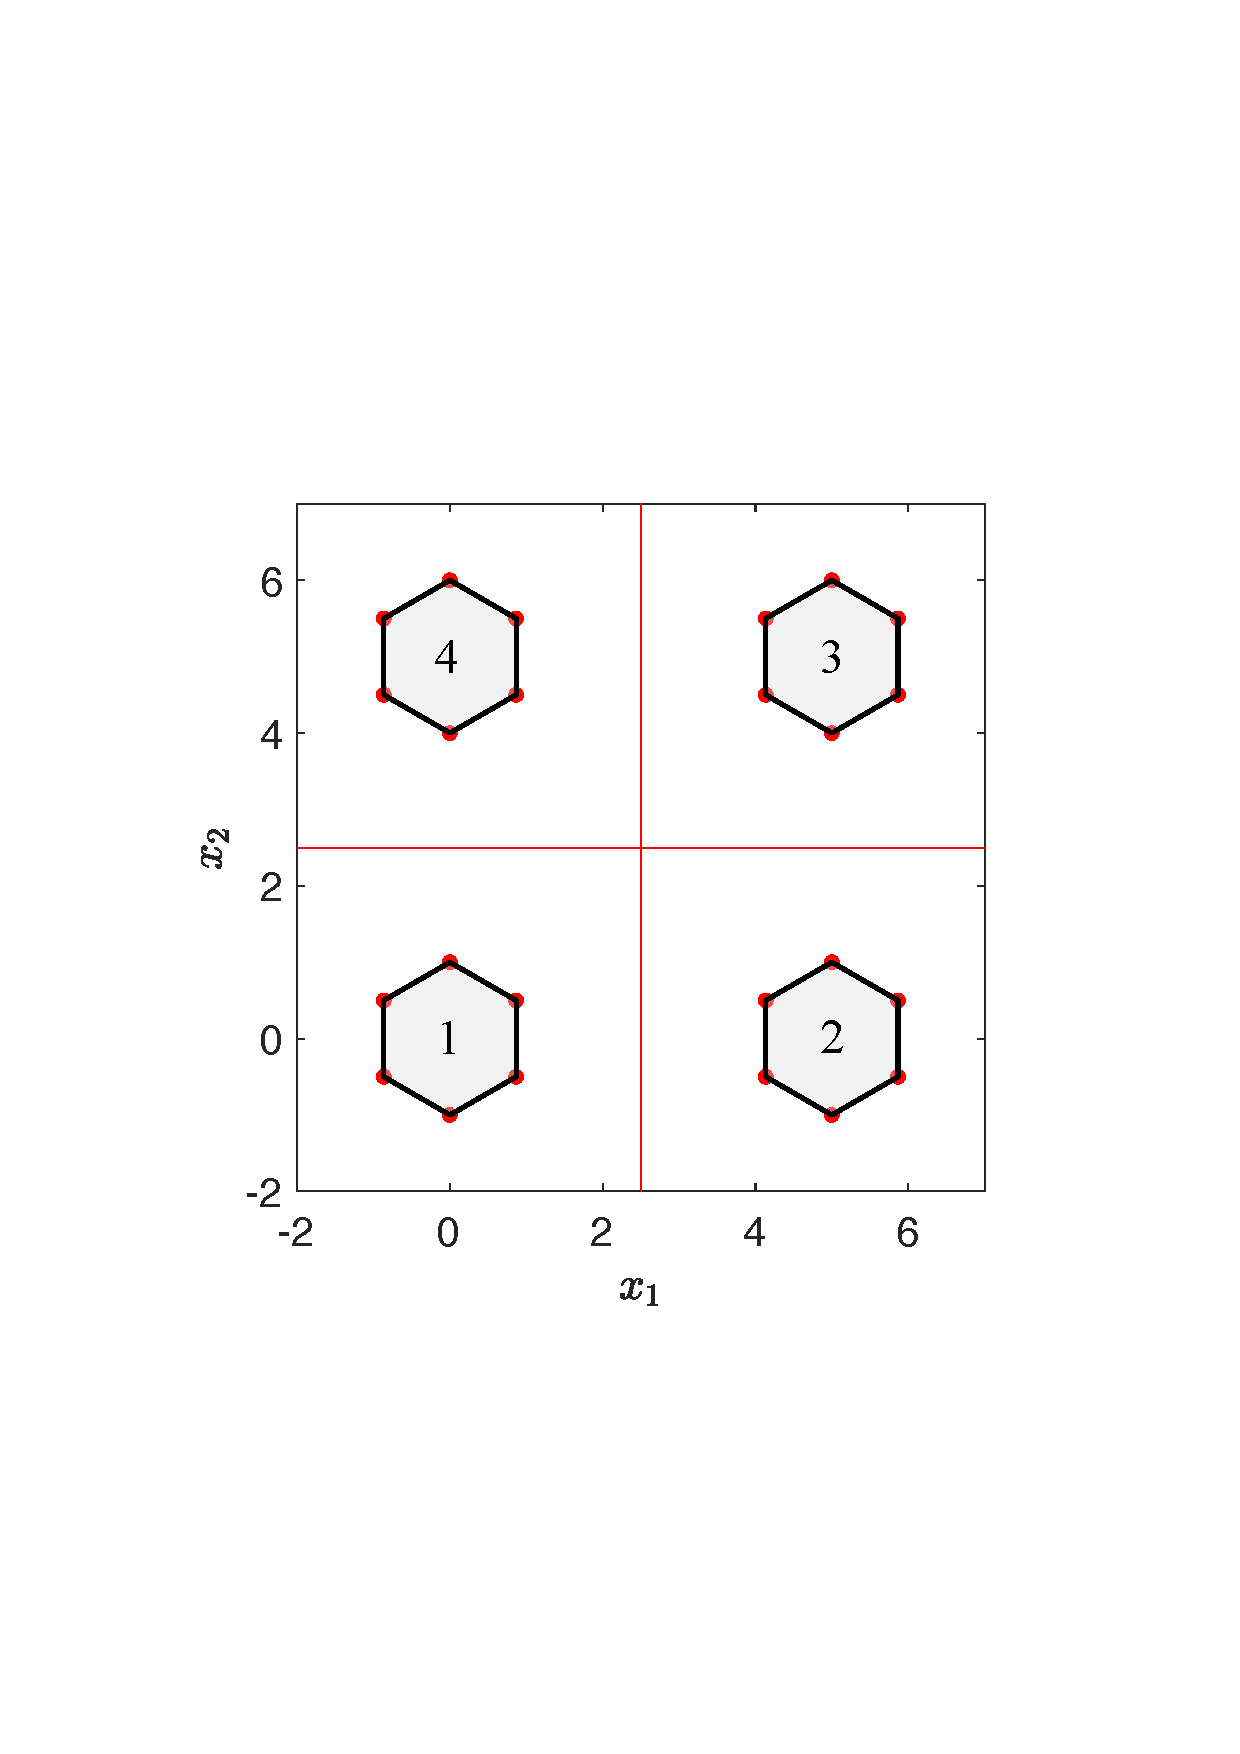
\includegraphics[width=.3\textwidth]{Section3/Alleles}
    \caption{Subdivision of the decision space of a multi-polygon problem into four parts. Each part can be viewed as an allele.}
    \label{fig: Alleles}
\end{figure}

\subsection{Crossover and mutation}
In evolutionary algorithms, crossover and mutation are two operators that can increase the diversity of the population. These two operators can help the algorithm to avoid trapping in the local optima. However, mutation and crossover are also likely to produce offspring that are close to their parents. More specifically, more offspring will be produced in the region where the parent population has high density. Fig. \ref{fig: SBX crossover} demonstrates the results of generating 1,000 individuals by the SBX\cite{deb1995simulated} crossover with distribution index = 20. As shown in Fig. \ref{fig: SBX crossover} (\subref{fig: SBX crossover case 1}) with two parents at $(0, 0)^T$ and $(5, 0)^T$, the diversity of solutions in the decision space does not change too much since no new solutions are generated in other polygons. In Fig. \ref{fig: SBX crossover} (\subref{fig: SBX crossover case 2}), the parents are two solutions in diagonal polygons, i.e. $(0, 0)^T$ and $(5, 5)^T$. In this case, the diversity of solutions in the decision space increases significantly since the number of polygons with solutions increases from two to four. Fig. \ref{fig: Polynomial mutation} depicts the results of the polynomial mutation \cite{deb2014analysing} with distribution index = 20. The number of polygons with solutions is not changed by mutation. From these two simulation results, we can see that standard crossover and mutation operators cannot efficiently create a wide variety of new offspring in the decision space.
\begin{figure}[t!]
	\centering
	\begin{subfigure}[b]{.24\textwidth}
		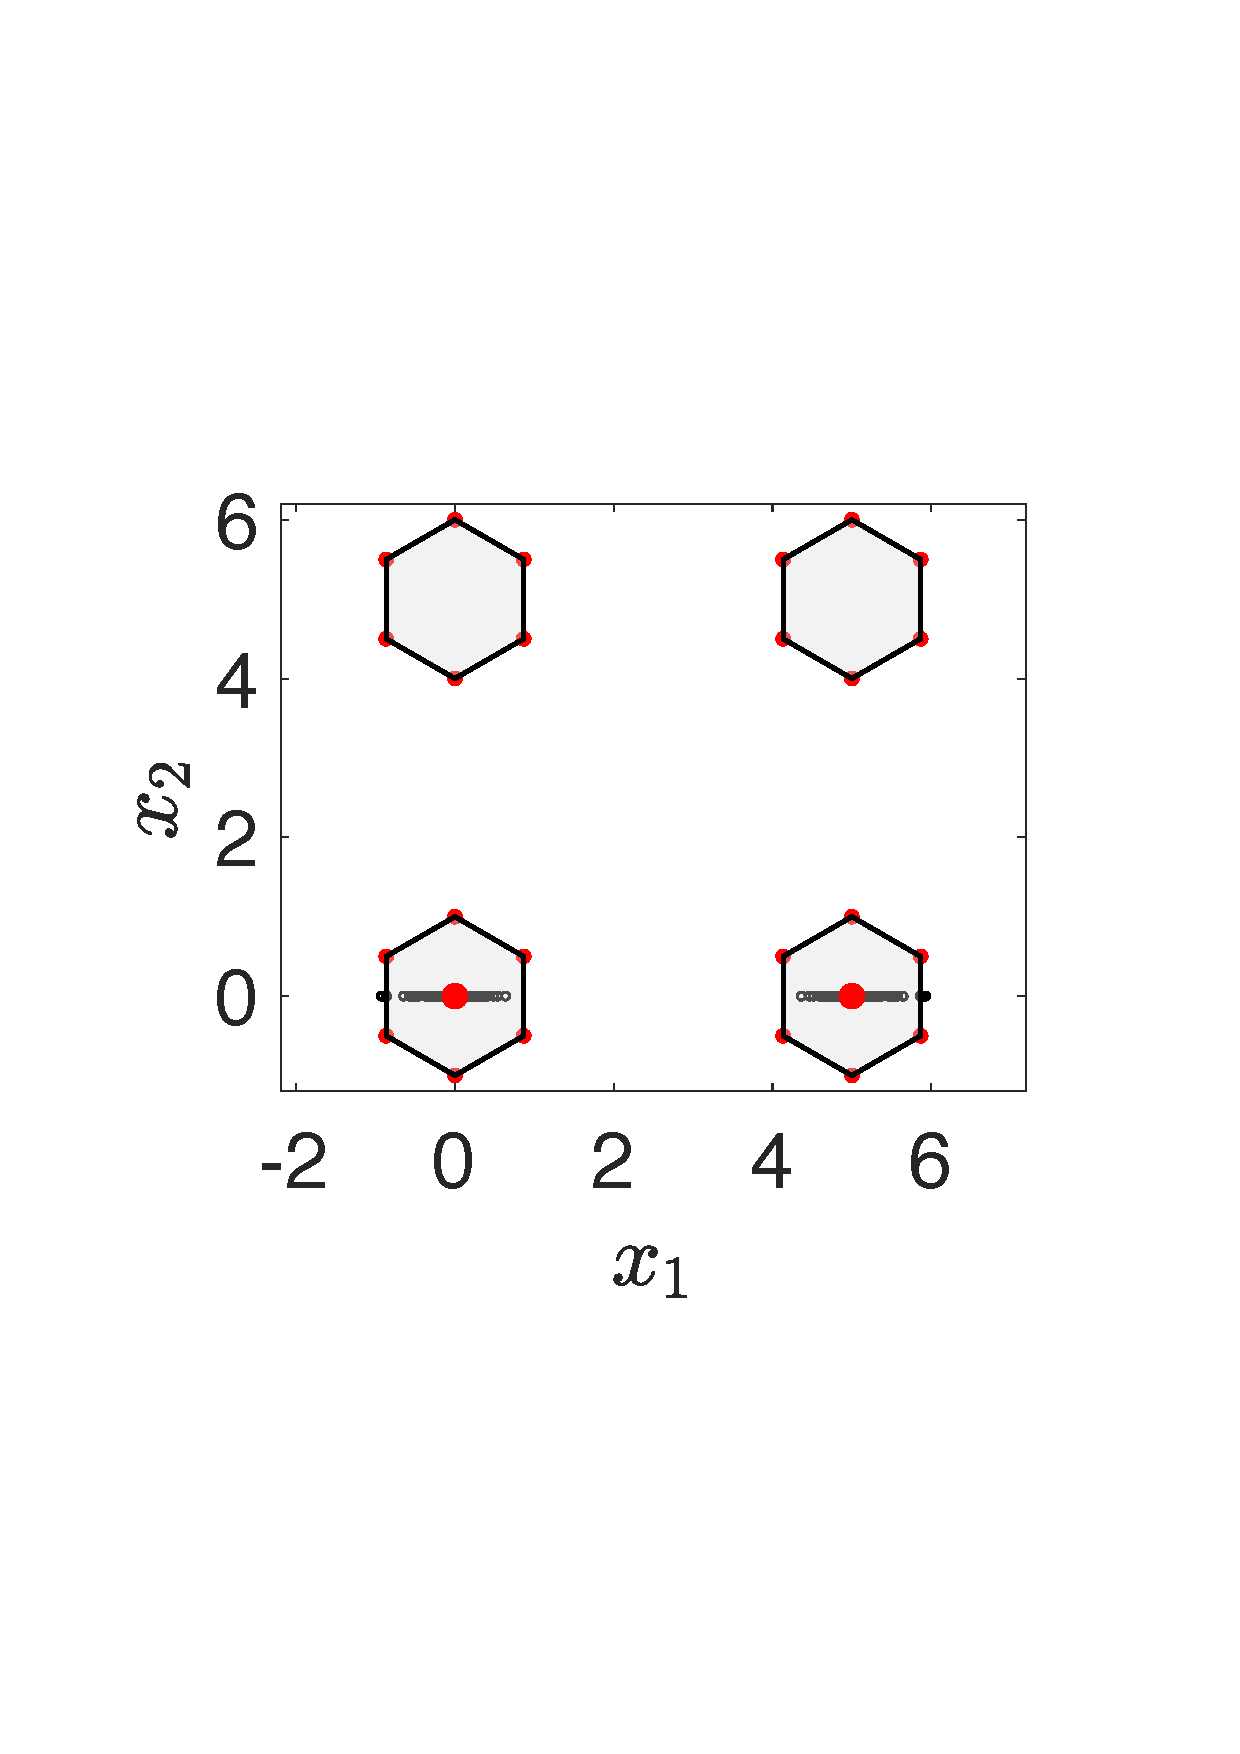
\includegraphics[width=\linewidth]{Section3/crossover1}
		\caption{Case 1: parents are $(0, 0)^T$ and $(5, 0)^T$.}
		\label{fig: SBX crossover case 1}
	\end{subfigure}
	\begin{subfigure}[b]{.24\textwidth}
		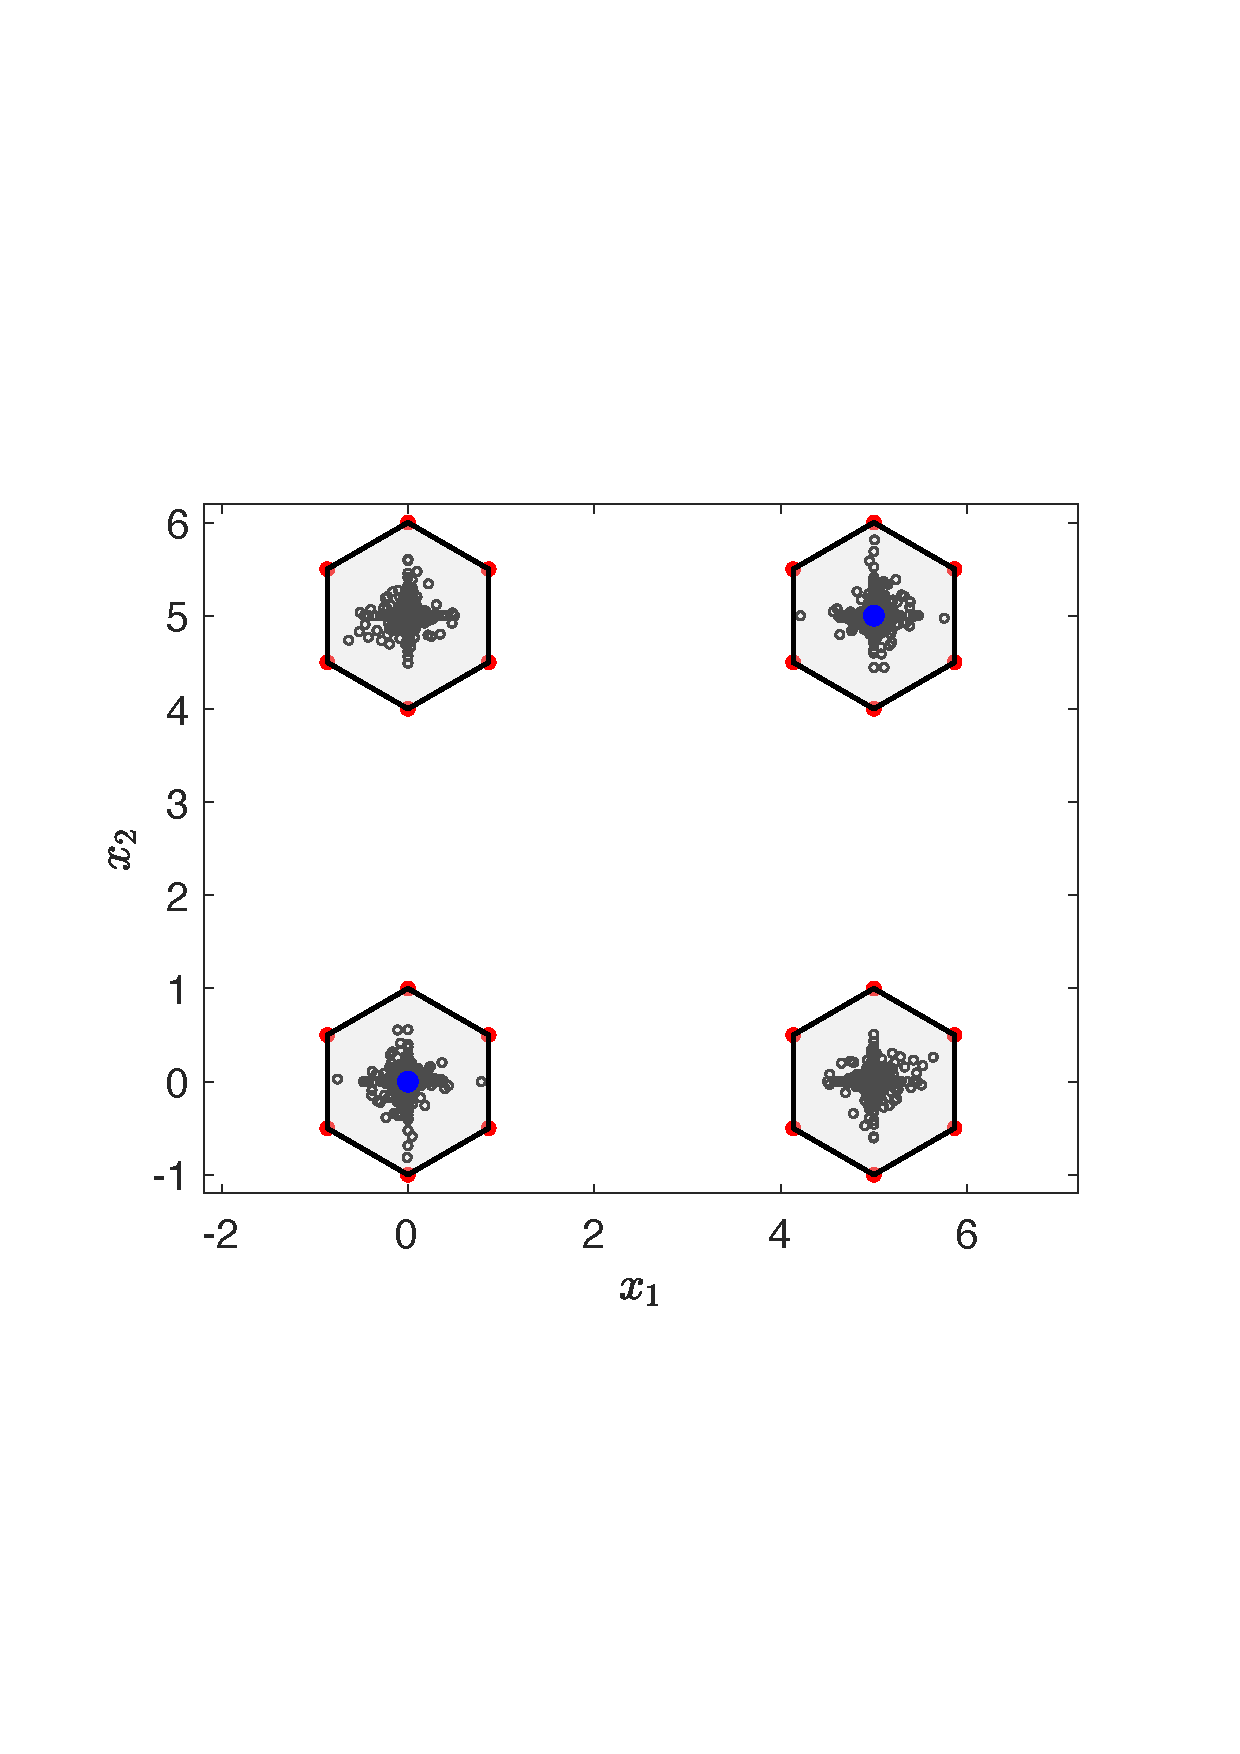
\includegraphics[width=\linewidth]{Section3/crossover2}
		\caption{Case 2: parents are $(0, 0)^T$ and $(5, 5)^T$.}
		\label{fig: SBX crossover case 2}
	\end{subfigure}
	\caption{Generated 1,000 offspring by the SBX crossover. Yellow and dark circles represent parent and offspring, respectively.}
	\label{fig: SBX crossover}
\end{figure}

\begin{figure}[t!]
    \centering
    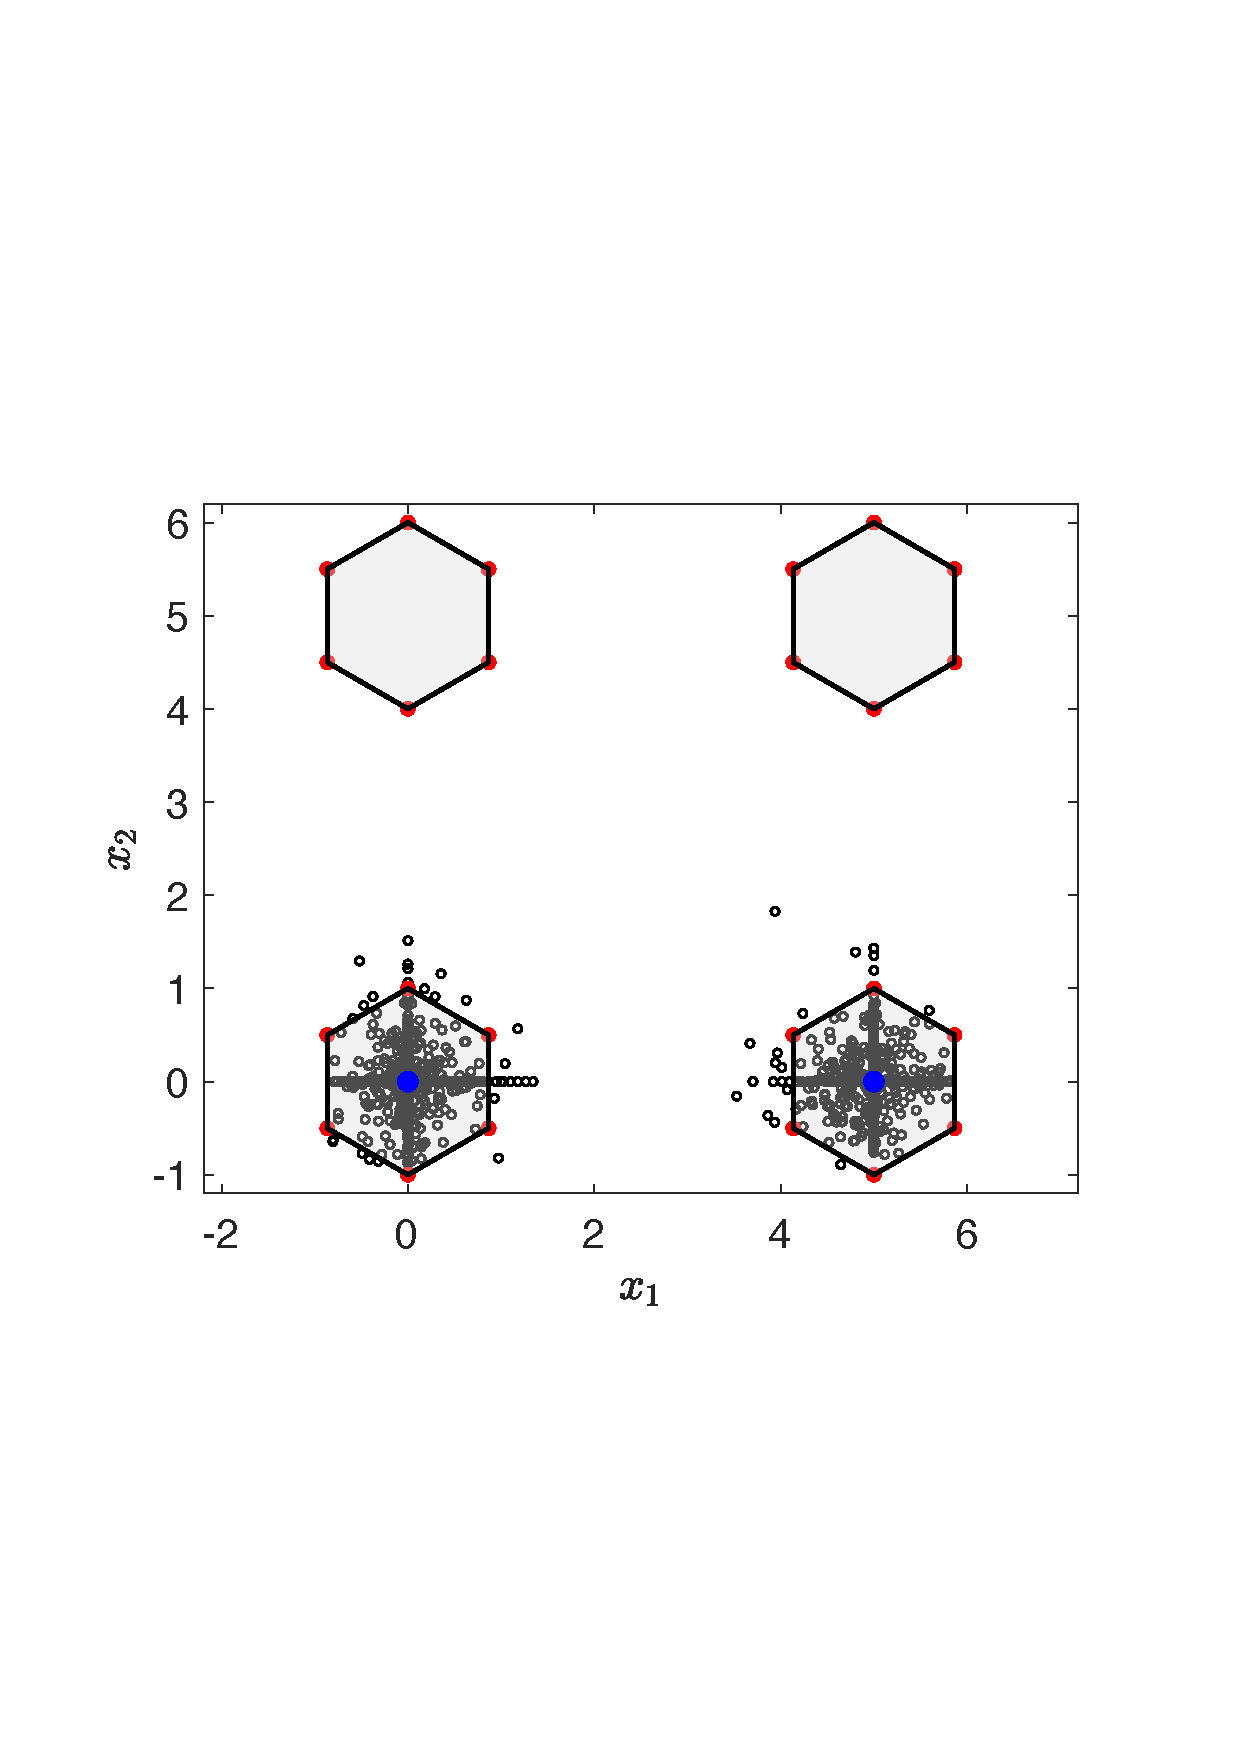
\includegraphics[width=.24\textwidth]{Section3/mutation}
    \caption{Generate 1,000 offspring by applying polynomial mutation to two solutions. Yellow and dark circles represent parent and offspring respectively.}
    \label{fig: Polynomial mutation}
\end{figure}
From the discussions above, we can see that additional diversity maintenance techniques are needed in MOEAs in their applications to MMOPs.

\section{Experimental Studies}

\label{Experimental Studies}
\subsection{Experimental settings}
\label{Experimental Settings}
\subsubsection{Algorithms for Comparison}
We select representative MOEAs from the following three classes:
\begin{itemize}
    \item \textbf{Pareto-dominance based}: NSGA-II\cite{deb2002fast}, and SPEA2\cite{zitzler2001spea2}.
    \item \textbf{Decomposition based}: MOEA/D \cite{zhang2007moea} with PBI ($\theta=5$) and Tchebycheff aggregation function and NSGA-III\cite{deb2013evolutionary}.
    \item \textbf{Indicator based}: IBEA\cite{zitzler2004indicator}.
\end{itemize}

We also used MMEAs mentioned in Subsection \ref{Review of State-of-the-art Techniques}: DNEA\cite{liu2018double}, MO\_Ring\_PSO\_SCD\cite{yue2017multiobjective}, MOEA/D-AD\cite{tanabe2018decomposition} and Omni-Optimizer\cite{deb2005omni}.
\subsubsection{Parameter Settings}
In our experiments, we use the following parameter settings: 
\paragraph{Test Problem Settings}
\begin{itemize}
     \item Number of objectives: $M=6$.
    \item Number of decision variables: $D=2, 4, 6, 8, 10, 100$.
    \item Four regular polygons with radius $r=1$ and centers $\boldsymbol{c}_1=(0, 0)^T$, $\boldsymbol{c}_2=(5, 0)^T$, $\boldsymbol{c}_3=(5, 5)^T$, $\boldsymbol{c}_4=(0, 5)^T$. 
\end{itemize}
\paragraph{Common Settings over All Algorithms:}
\begin{itemize}
    \item Population size: $N$ = 300.
    \item Number of evaluations = $10^5$.
    \item SBX crossover: distribution index = 20 and crossover probability = 1.0.
    \item Polynomial mutation:  distribution index = 20) and mutation probability $1/D$.
\end{itemize}
\paragraph{Specific Settings for Each Algorithm}
We use default parameters for each algorithm according to the corresponding paper.
\begin{itemize}
    \item IBEA. Fitness scaling factor: $\kappa=0.05$.
    \item DNEA. Niche radius in the objective space: $\delta_{obj}=0.06$; Niche radius in the decision space $\delta_{var}=0.02$.
    \item MO\_Ring\_PSO\_SCD. Archive size: $n_{\text{PBA}}=5$ for the personal best archive, $n_{\text{NBA}}=15$ for the neighborhood best archive.
    \item MOEA/D-AD. Use PBI ($\theta=5$) aggregation function and neighborhood size $L = \lfloor 0.1\mu \rfloor$ where $\mu$ is the size of current population.
    \item Omni-optimizer. $\epsilon$-dominance parameter: $\delta=0.001$.
\end{itemize}

\subsection{Experimental results and analysis}
\label{Experimental Results}
In this section, we examine the performance of the selected MOEAs and MMEAs on multi-polygon test problems using PlatEMO platform\cite{tian2017platemo}. In each experiment, each algorithm is executed 31 times. Then the one with the median HV among them is chosen as representative. In a similar manner to \cite{ishibuchi2019salable}, we plot the two-dimensional projection of the obtained solutions to visualize their distribution in the decision space. We also evaluate the performance of MOEAs and MMEAs in the objective space.
%% dim = 2 PS plot 
\begin{figure}[t!]
    \centering
    \begin{subfigure}[b]{.24\textwidth}
    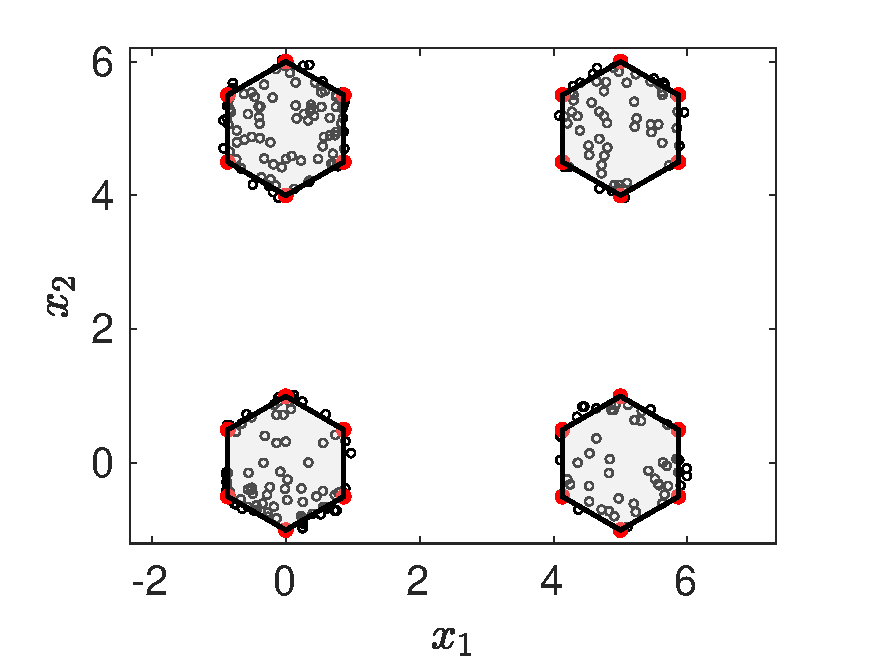
\includegraphics[width=\linewidth]{Section5/dim2/PS/NSGAII}
    \caption{NSGA-II}
    \end{subfigure}
    \begin{subfigure}[b]{.24\textwidth}
    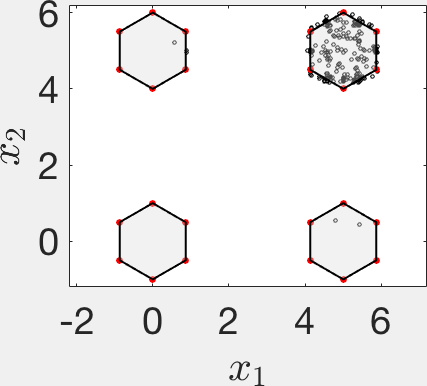
\includegraphics[width=\linewidth]{Section5/dim2/PS/NSGAIII}
    \caption{NSGA-III}
    \end{subfigure}
    
    \begin{subfigure}[b]{.24\textwidth}
    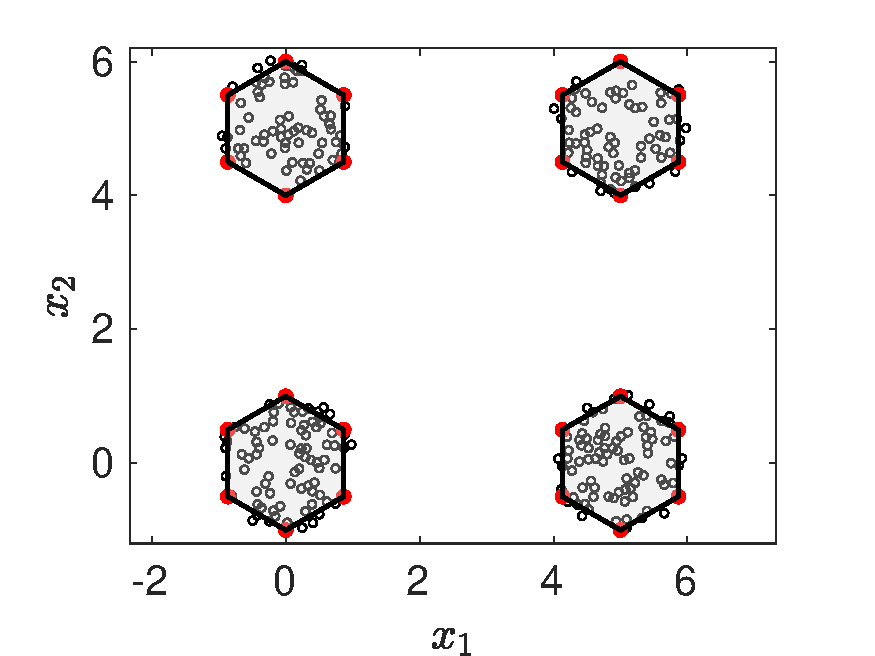
\includegraphics[width=\linewidth]{Section5/dim2/PS/SPEA2}
    \caption{SPEA2}
    \end{subfigure}
    \begin{subfigure}[b]{.24\textwidth}
    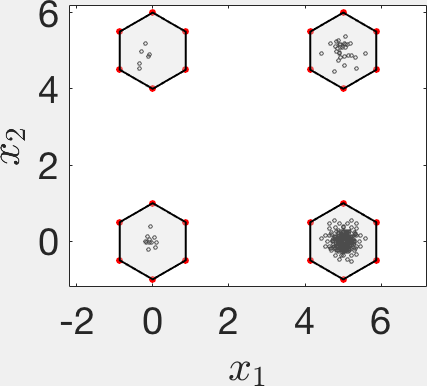
\includegraphics[width=\linewidth]{Section5/dim2/PS/MOEAD_TCH}
    \caption{MOEA/D-TCH}
    \end{subfigure}
    
    \begin{subfigure}[b]{.24\textwidth}
    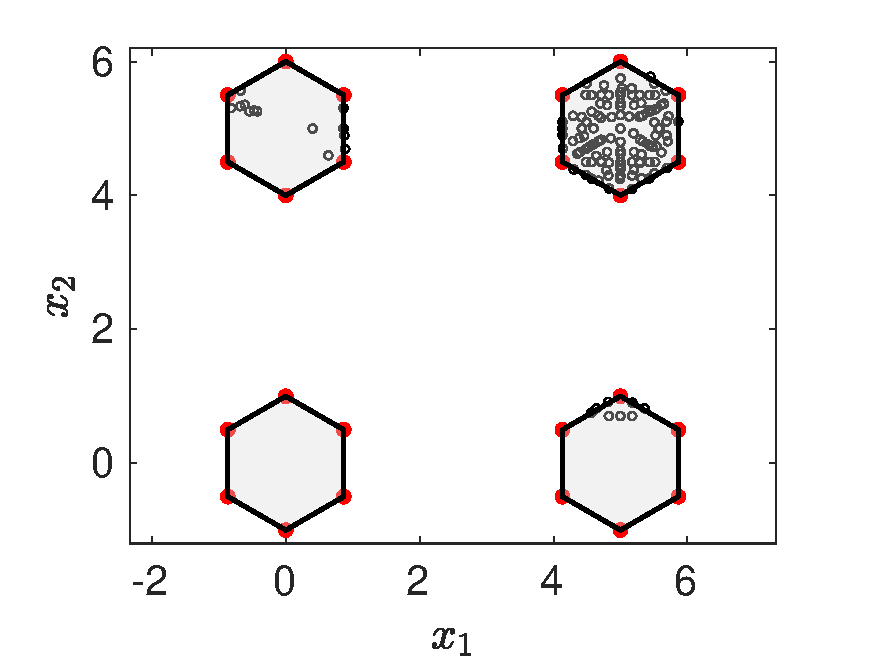
\includegraphics[width=\linewidth]{Section5/dim2/PS/MOEAD_PBI}
    \caption{MOEA/D-PBI}
    \end{subfigure}
    \begin{subfigure}[b]{.24\textwidth}
    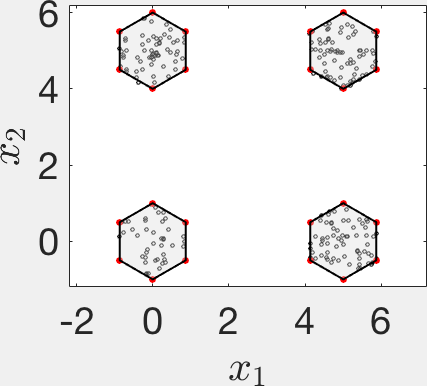
\includegraphics[width=\linewidth]{Section5/dim2/PS/IBEA}
    \caption{IBEA}
    \end{subfigure}

    \caption{Simulation results of MMEAs on multi-polygon test problem with $D=2$.}
    \label{fig: MOEAs PS dim=2}
\end{figure}

\begin{figure}[t!]
    \centering
    \begin{subfigure}[b]{.24\textwidth}
    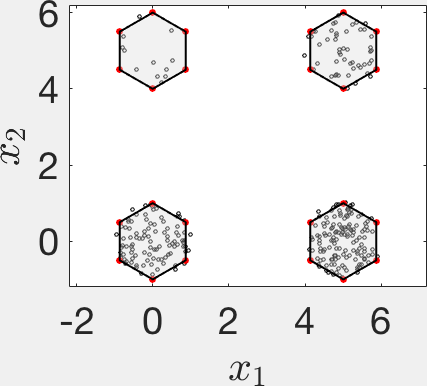
\includegraphics[width=\linewidth]{Section5/dim2/PS/DNEA}
    \caption{DNEA}
    \end{subfigure}
    \begin{subfigure}[b]{.24\textwidth}
    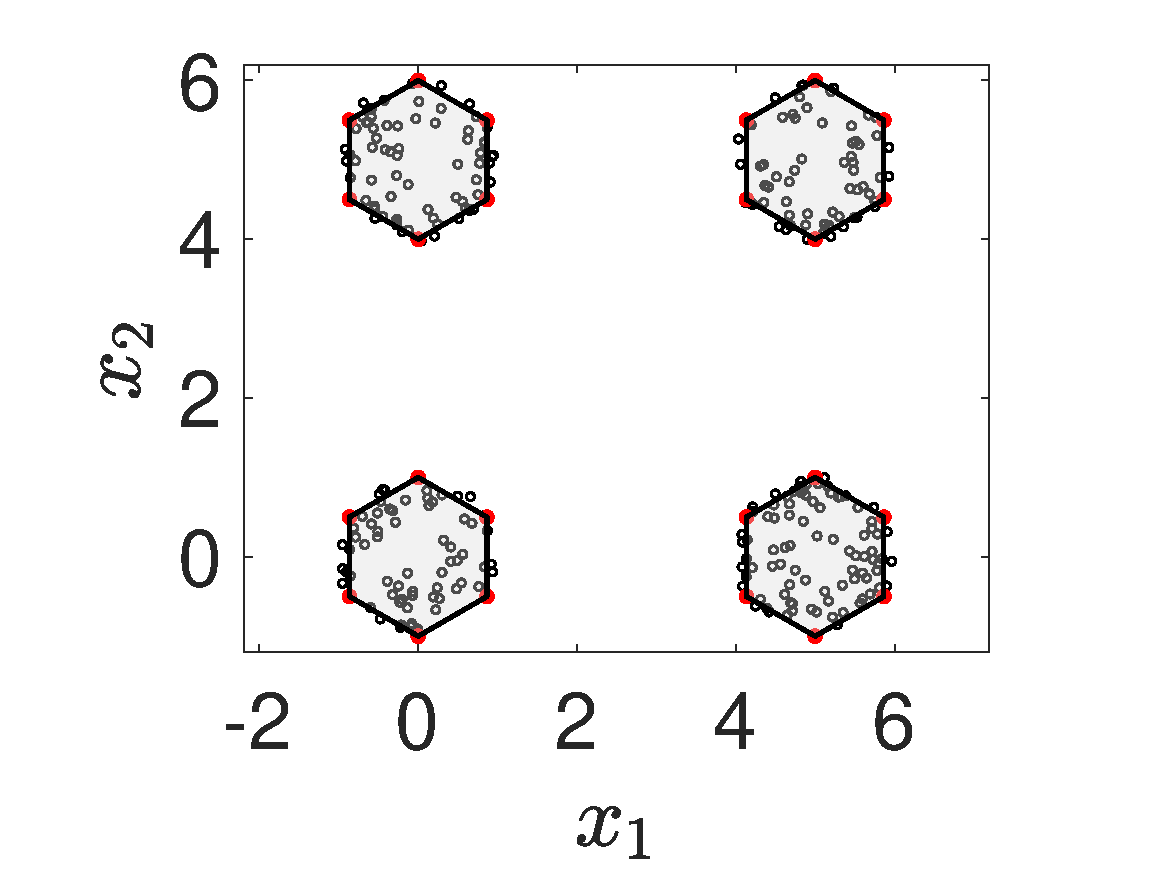
\includegraphics[width=\linewidth]{Section5/dim2/PS/MO_Ring_PSO_SCD}
    \caption{MO\_Ring\_PSO\_SCD}
    \end{subfigure}
    
    \begin{subfigure}[b]{.24\textwidth}
    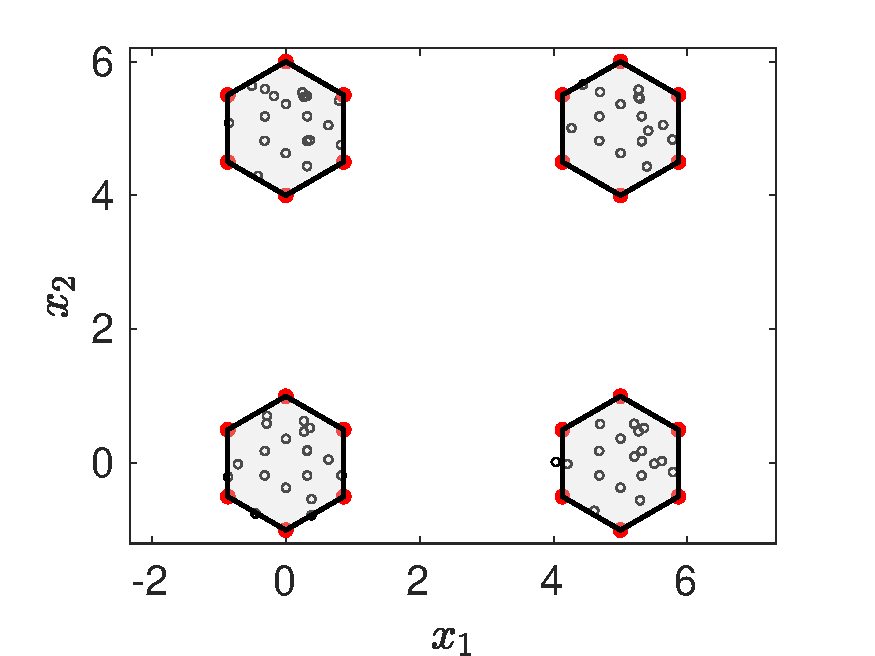
\includegraphics[width=\linewidth]{Section5/dim2/PS/MOEADAD}
    \caption{MOEA/D-AD}
    \end{subfigure}
    \begin{subfigure}[b]{.24\textwidth}
    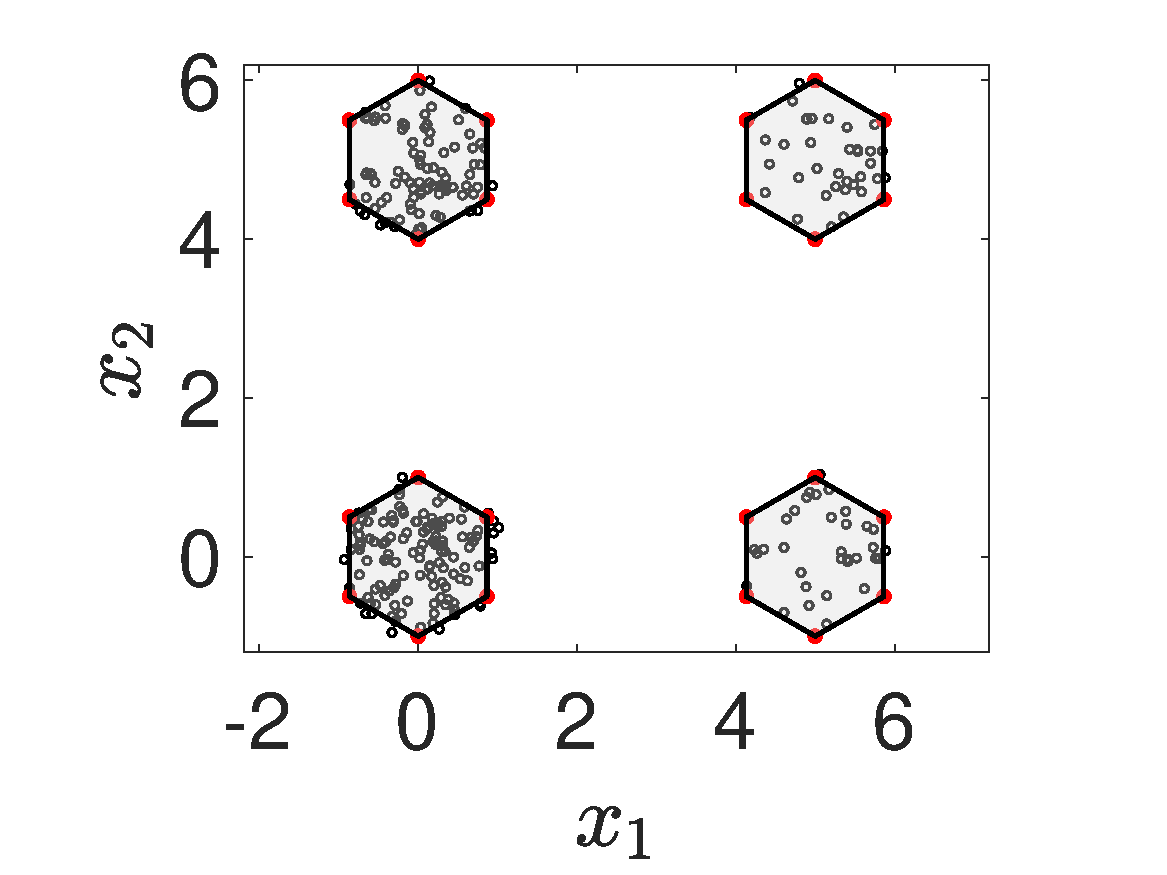
\includegraphics[width=\linewidth]{Section5/dim2/PS/OmniOptimizer}
    \caption{Omni-optimizer}
    \end{subfigure}
    \caption{Simulation results of MMEAs on multi-polygon test problem with $D=2$.}
    \label{fig: MMEAs PS dim=2}
\end{figure}

Figs. \ref{fig: MOEAs PS dim=2} and \ref{fig: MMEAs PS dim=2} show the simulation results of MOEAs and MMEAs when $D=2$. It is shown that MOEA/D and NSGA-III perform poorer than the other algorithms as MMEAs in Fig. \ref{fig: MOEAs PS dim=2}. When $D=2$, all algorithms except MOEA/D and NSGA-III can obtain a good coverage of the true Pareto sets in the decision space.

As discussed in section \ref{Difficulties Analysis}, MOEAs usually do not work well on MMOPs. However, the experimental results in Fig. \ref{fig: MOEAs PS dim=2} are good. In order to examine the reason, we divide the decision space into four parts, and mark them as area 1\textasciitilde 4  as shown in Fig. \ref{fig: Alleles}. Then, after every 500 evaluations, the number of solutions in each area is recorded. In addition, the IGD value is also recorded to show the evolutionary progress. 

%% dim = 2 Diversity Plot
\begin{figure}[t!]
    \centering
    \begin{subfigure}[b]{.24\textwidth}
    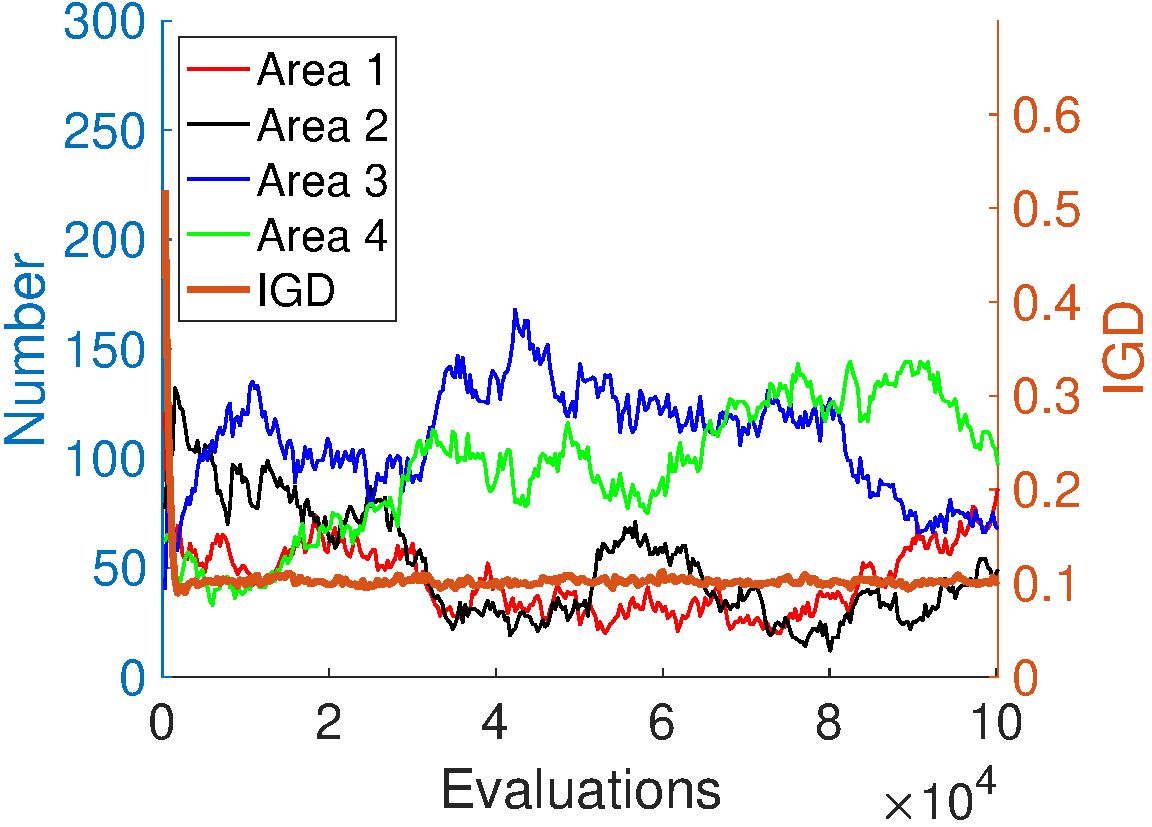
\includegraphics[width=\linewidth]{Section5/dim2/Diversity/NSGAII}
    \caption{NSGA-II}
    \end{subfigure}
    \begin{subfigure}[b]{.24\textwidth}
    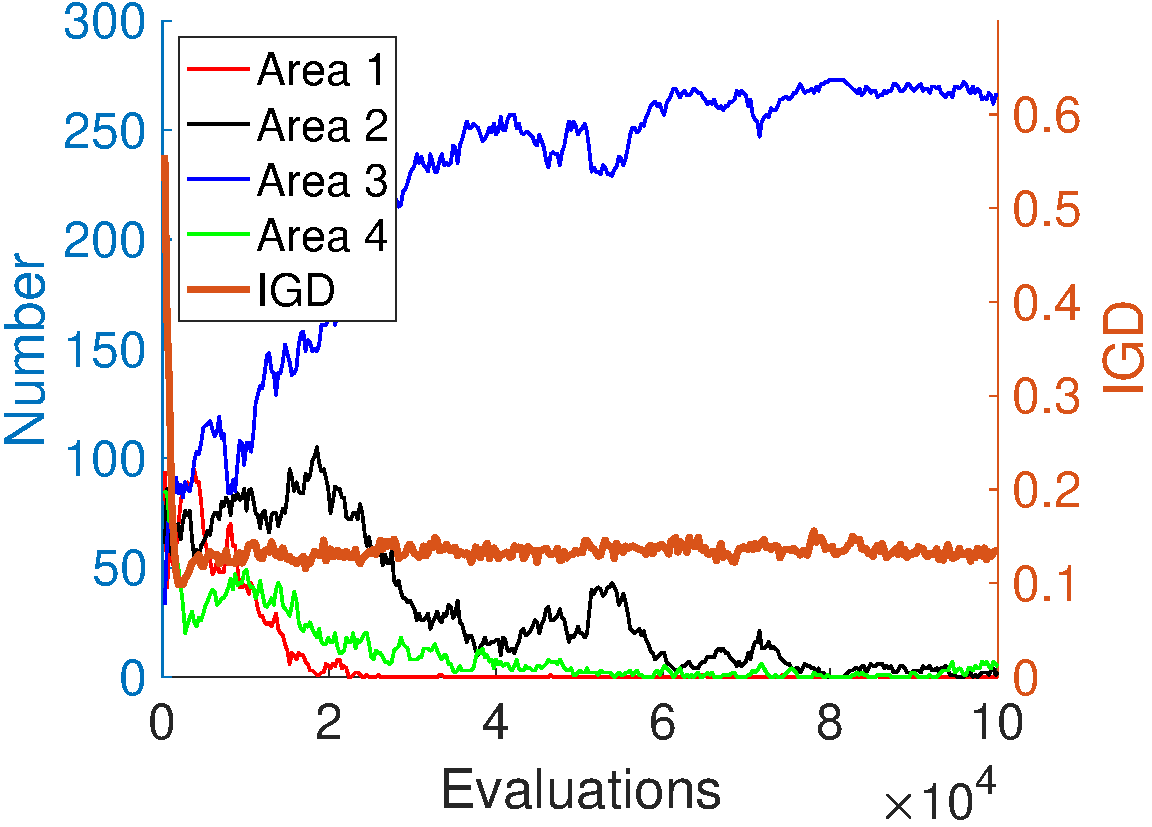
\includegraphics[width=\linewidth]{Section5/dim2/Diversity/NSGAIII}
    \caption{NSGA-III}
    \label{fig: NSGA-III Diversity dim=2}
    
    \end{subfigure}
    \begin{subfigure}[b]{.24\textwidth}
    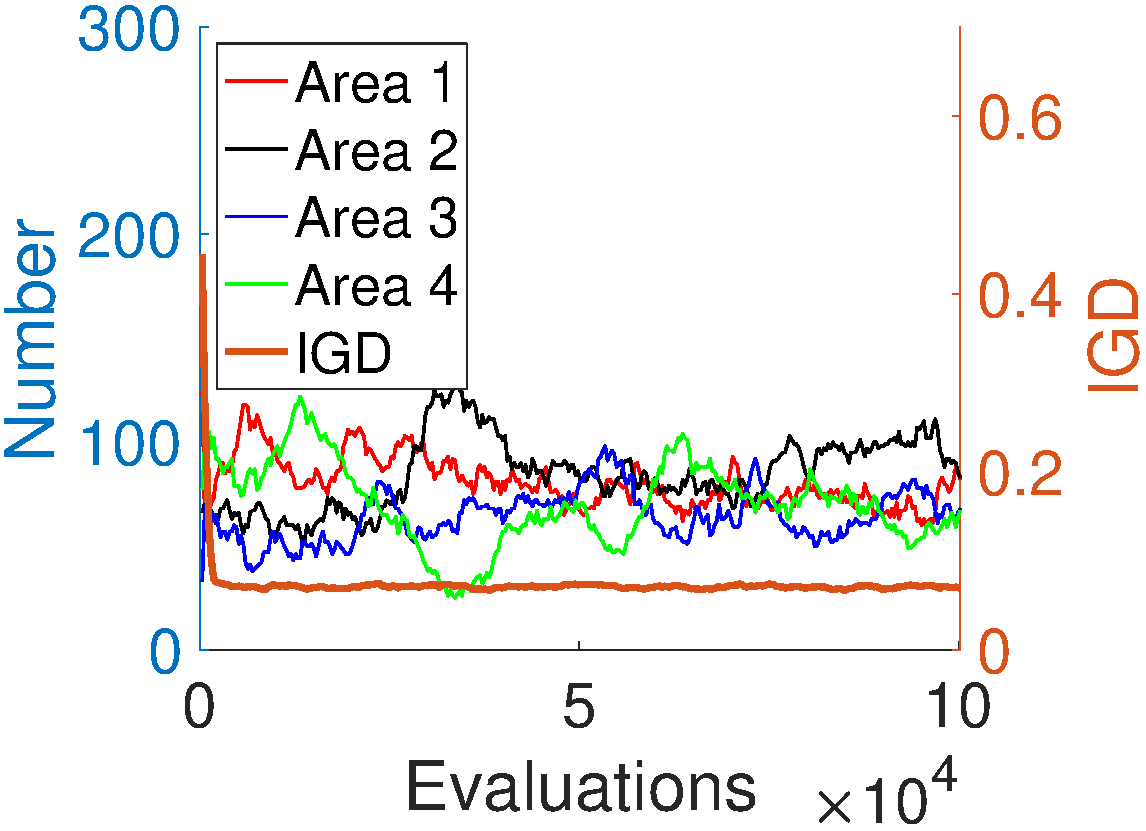
\includegraphics[width=\linewidth]{Section5/dim2/Diversity/SPEA2}
    \caption{SPEA2}
    \end{subfigure}
    \begin{subfigure}[b]{.24\textwidth}
    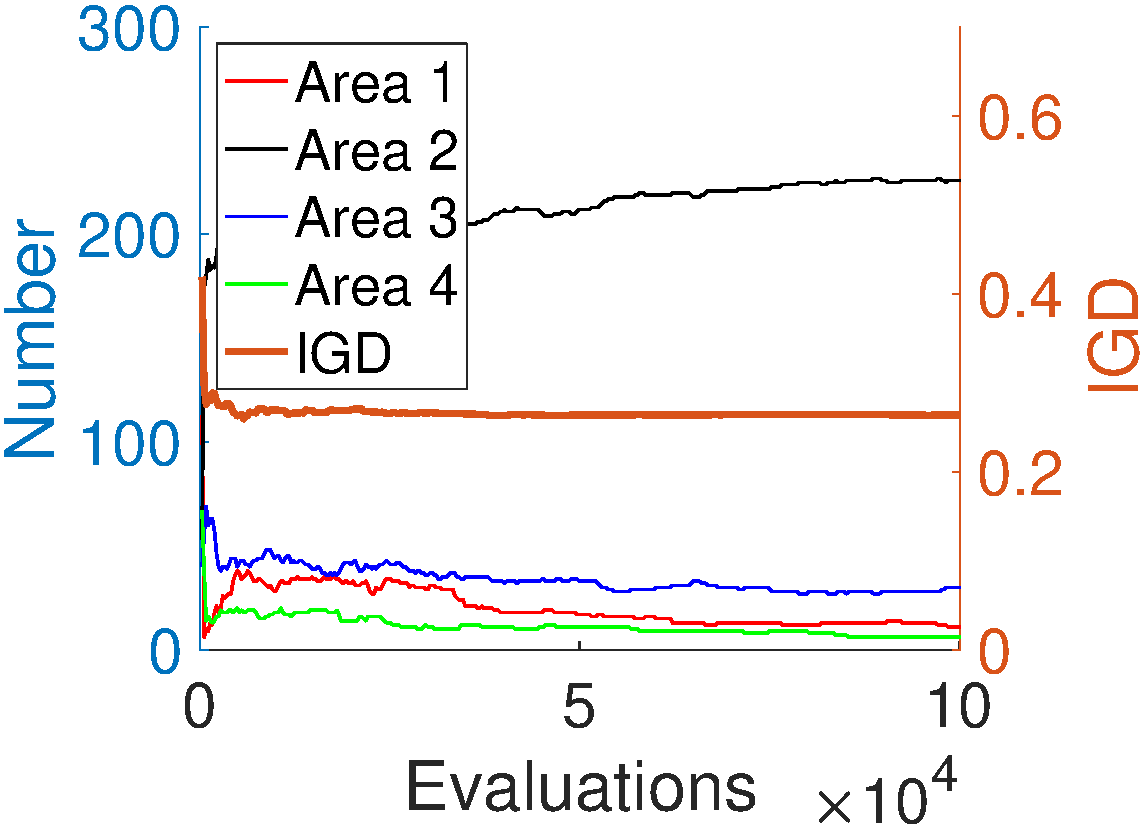
\includegraphics[width=\linewidth]{Section5/dim2/Diversity/MOEAD_TCH}
    \caption{MOEA/D-TCH}
    \label{fig: MOEA/D-TCH Diversity dim=2}
    \end{subfigure}
    
    \begin{subfigure}[b]{.24\textwidth}
    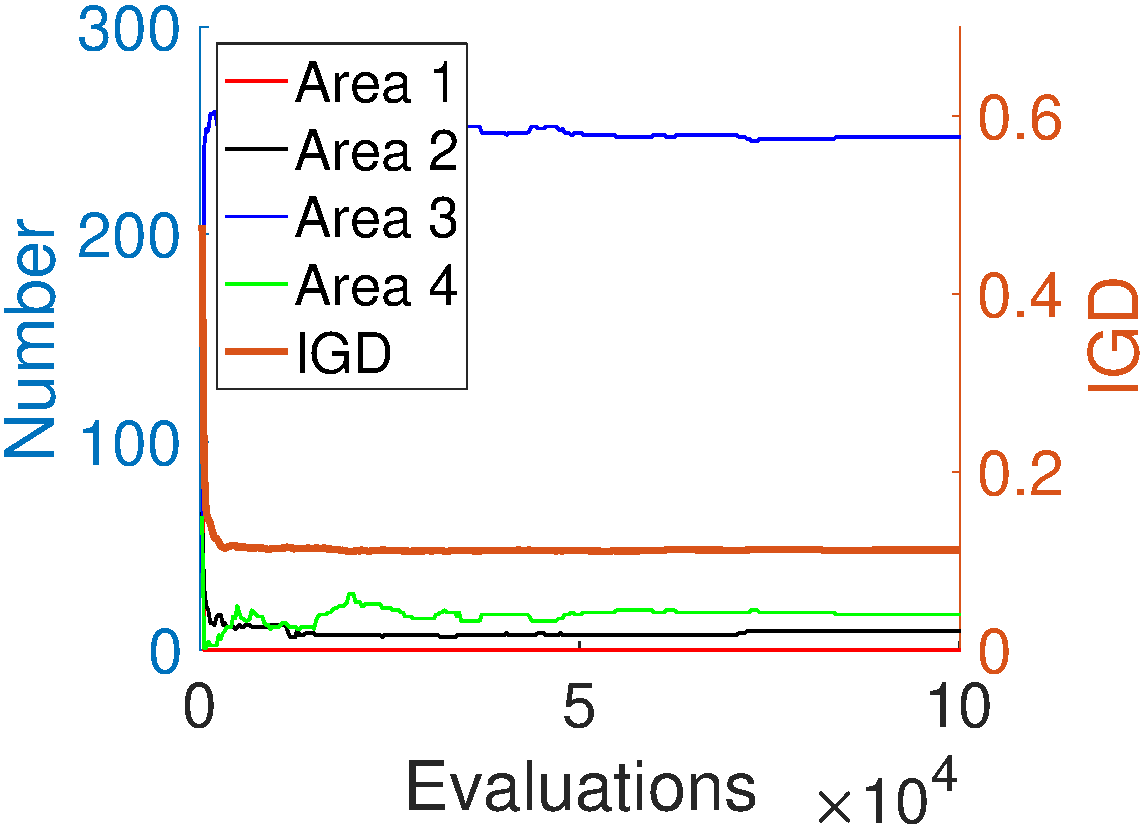
\includegraphics[width=\linewidth]{Section5/dim2/Diversity/MOEAD_PBI}
    \caption{MOEA/D-PBI}
    \label{fig: MOEA/D-PBI Diversity dim=2}
    \end{subfigure}
    \begin{subfigure}[b]{.24\textwidth}
    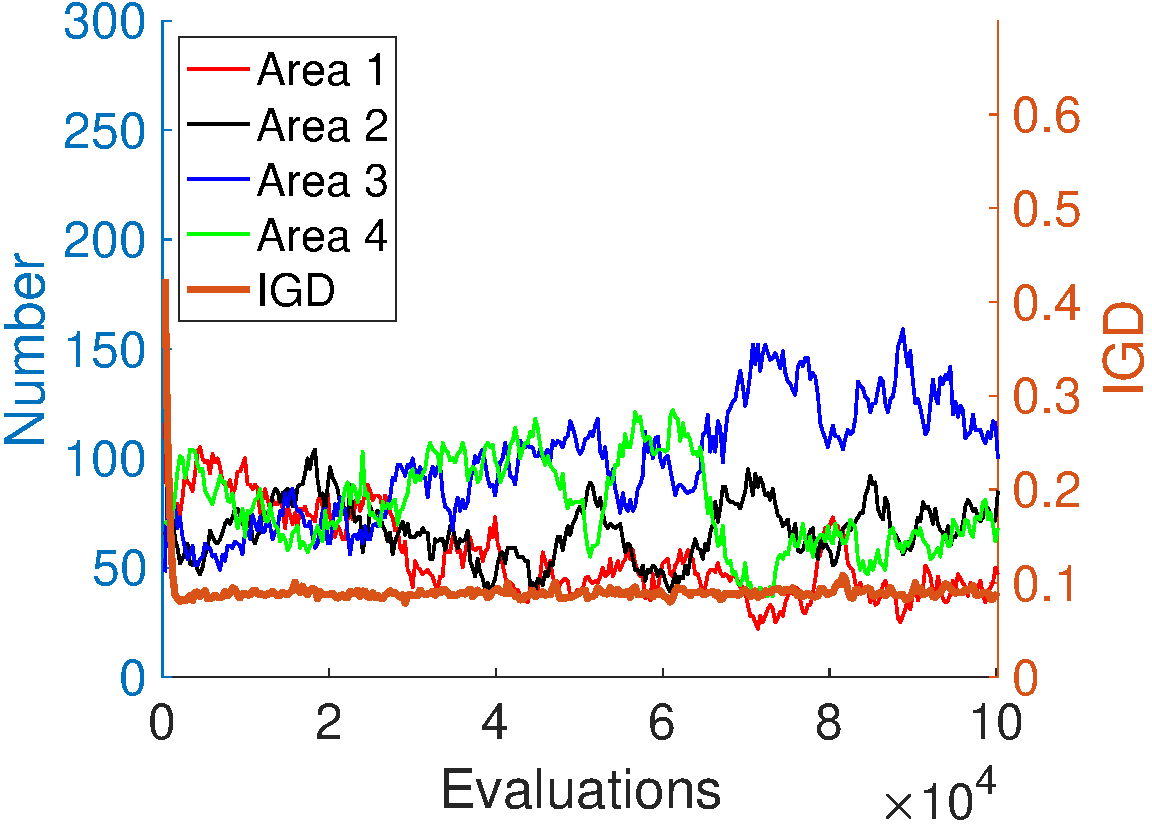
\includegraphics[width=\linewidth]{Section5/dim2/Diversity/IBEA}
    \caption{IBEA}
    \end{subfigure}

    \caption{The number of solutions in each area and the IGD value through the evolution by each MOEA on the multi-polygon test problem with $D=2$.}
    \label{fig: MOEAs Diversity dim=2}
\end{figure}

\begin{figure}[t!]
    \centering
    \begin{subfigure}[b]{.24\textwidth}
    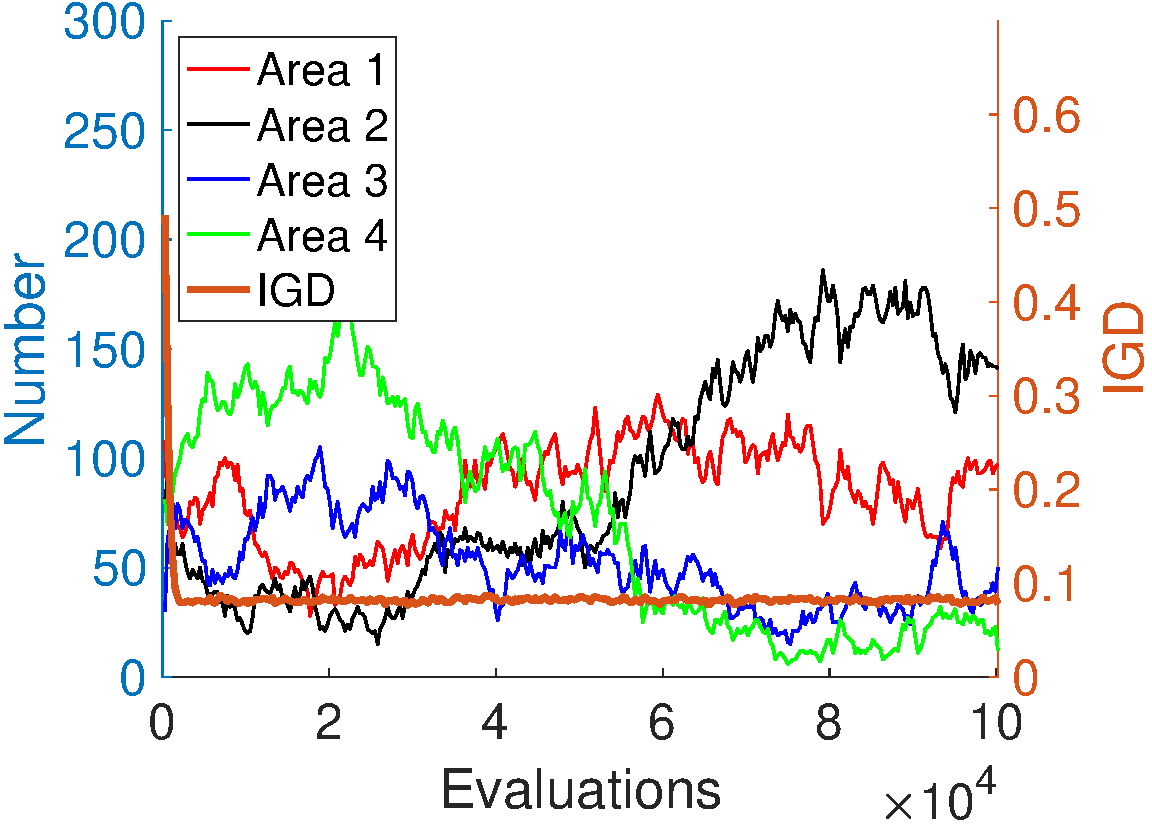
\includegraphics[width=\linewidth]{Section5/dim2/Diversity/DNEA}
    \caption{DNEA}
    \end{subfigure}
    \begin{subfigure}[b]{.24\textwidth}
    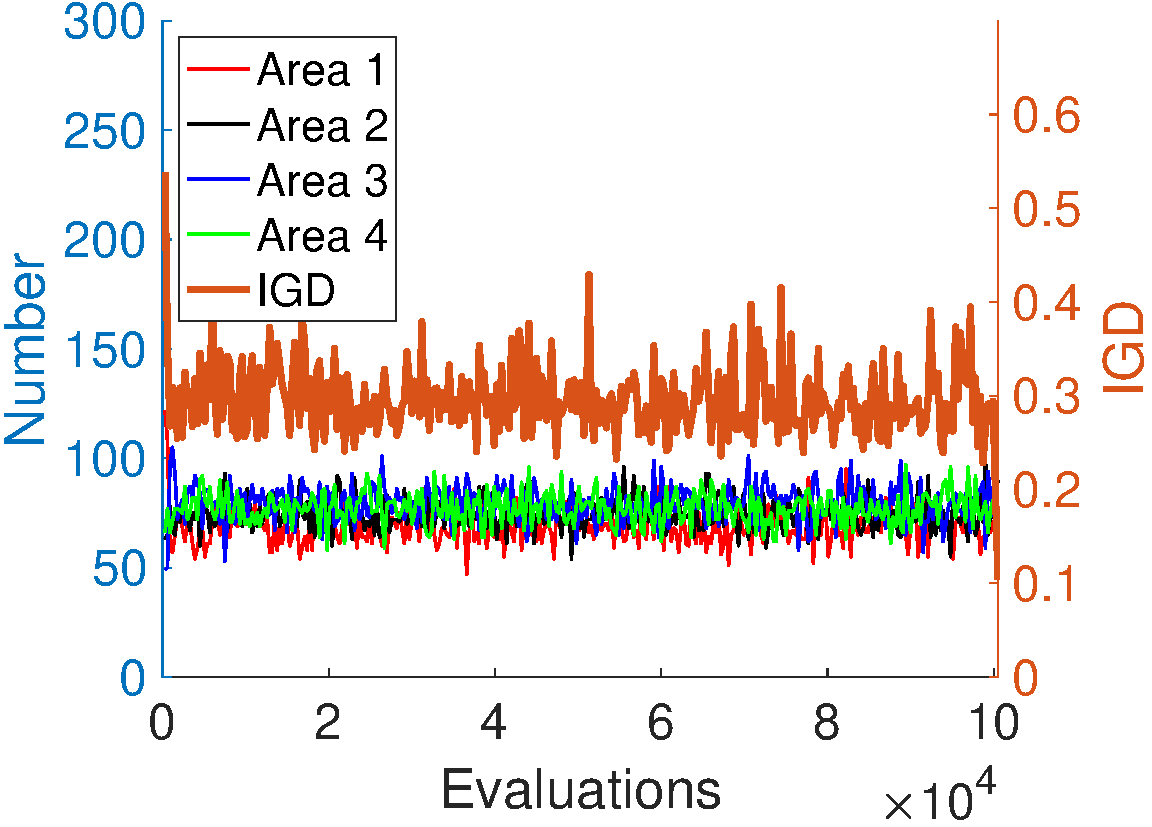
\includegraphics[width=\linewidth]{Section5/dim2/Diversity/MO_Ring_PSO_SCD}
    \caption{MO\_Ring\_PSO\_SCD}
    \end{subfigure}
    
    \begin{subfigure}[b]{.24\textwidth}
    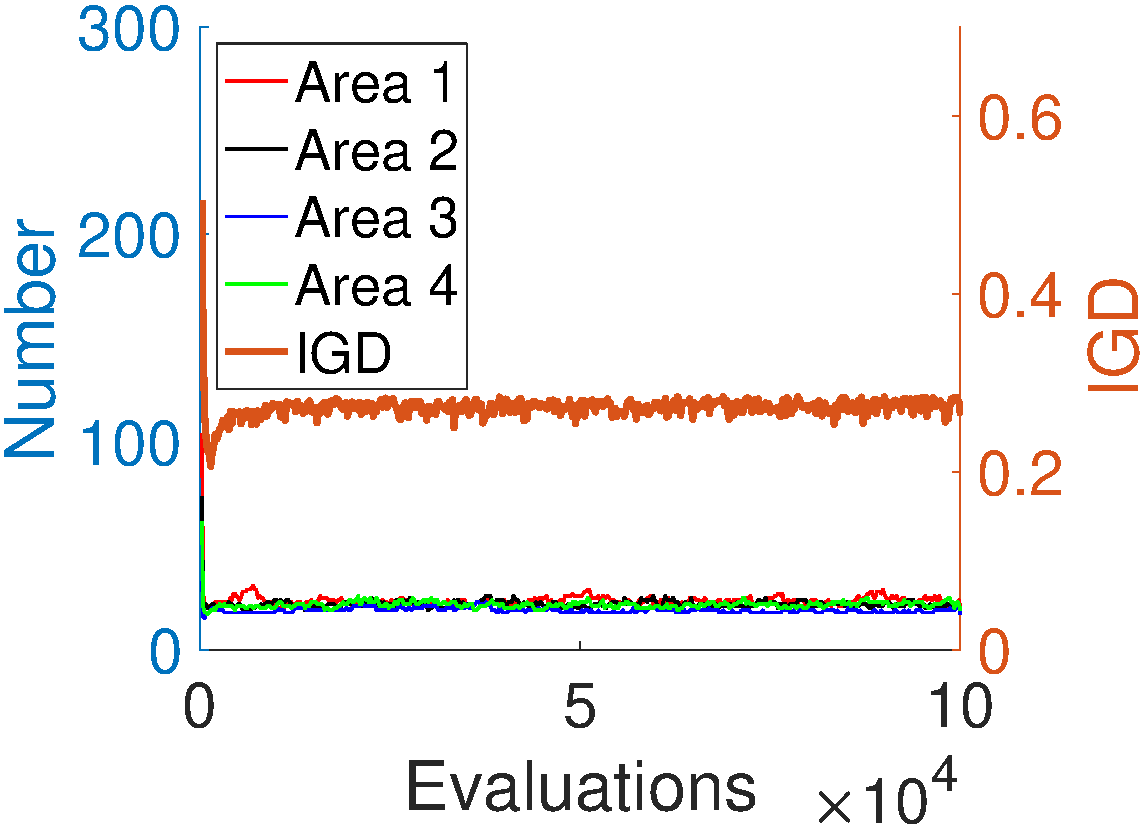
\includegraphics[width=\linewidth]{Section5/dim2/Diversity/MOEADAD}
    \caption{MOEA/D-AD}
    \end{subfigure}
    \begin{subfigure}[b]{.24\textwidth}
    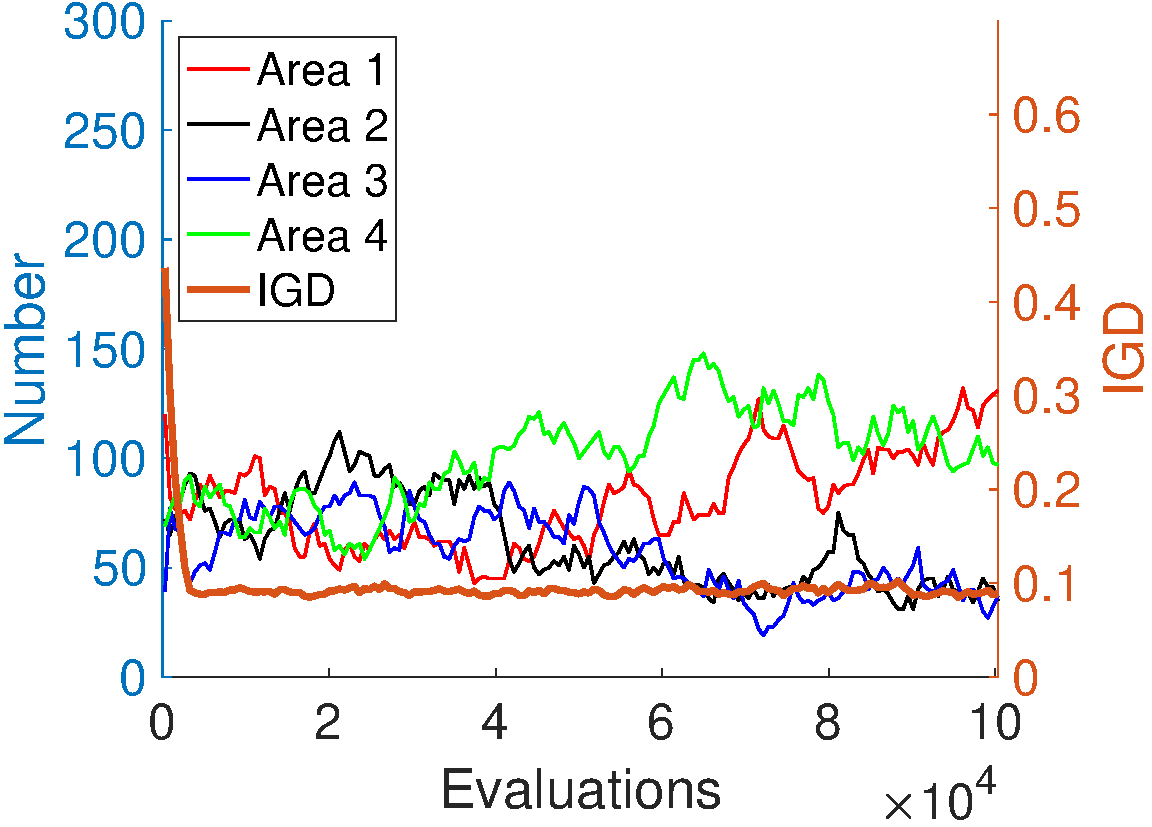
\includegraphics[width=\linewidth]{Section5/dim2/Diversity/OmniOptimizer}
    \caption{Omni-optimizer}
    \end{subfigure}
    \caption{The number of solutions in each area and the IGD value through the evolution by each MMEA on the multi-polygon test problem with $D=2$.}
    \label{fig: MMEAs Diversity dim=2}
\end{figure}

Figs. \ref{fig: MOEAs Diversity dim=2} and \ref{fig: MMEAs Diversity dim=2} show the number of solutions in each area and the IGD value for MOEAs and MMEAs, respectively. According to Fig. \ref{fig: MOEAs Diversity dim=2}, the number of solutions in each area establishes a "dynamic balance" in the case of MOEAs which perform well on the test problem with $D=2$. As shown in Fig. \ref{fig: SBX crossover} (\subref{fig: SBX crossover case 2}), SBX crossover of two solutions in diagonal areas significantly improves the diversity of solutions in the decision space. When enough solutions exist both area in the diagonal position (i.e., areas 1 and 3 or areas 2 and 4), a dynamic balance is formed. However, when a single area has too many solutions and its diagonal position area does not have enough solutions, a dynamic balance is not formed. For example, in the case of NSGA-III in Fig. \ref{fig: MOEAs Diversity dim=2} (\subref{fig: NSGA-III Diversity dim=2}), although the diversity of solution is good in a very early stage of evolution, most solutions in the final population are in area 3. In Fig. \ref{fig: MOEAs Diversity dim=2}, the number of solutions in area 3 starts to quickly increase around the 10, 000th function evaluations. At the same time, the number of solutions in area 1 (i.e., the diagonal position of area 3) starts to quickly decrease. During the next 10, 000 evaluations, the number of solutions in area 1 becomes almost zero. As a result, no solutions in areas 2 and 4 can be generated by recombining solutions in area 1 and 3. Therefore, the number of solutions in area 2 and 4 gradually decreases after around 20, 000th evaluations. We have similar observations in Fig. \ref{fig: MOEAs Diversity dim=2} (d) and (e) by MOEA/D. Since NSGA-III has a similar environmental selection mechanism to MOEA/D, it is likely that decomposition-based algorithms have strong convergence property to a single Pareto set. As shown in Fig. \ref{fig: MMEAs PS dim=2} obtained by MMEAs, all areas have some solutions thanks to a diversity maintenance mechanism in each algorithm.

In the same manner, we examine the case with $D=4$ (i.e., the four-dimensional multi-polygon problem). The two-dimensional projection of the final population is shown in Figs. \ref{fig: MOEAs PS dim=4} and \ref{fig: MMEAs PS dim=4}. The experimental results reveal that the increase of the number of decision variables will quickly increase the difficulty to cover all polygons. In Fig. \ref{fig: MMEAs PS dim=4} by MMEAs, MO\_Ring\_PSO\_SCD and MOEA/D-AD are still able to obtain satisfactory results. However, DNEA and Omni-optimizer do not work well on Fig. \ref{fig: MMEAs PS dim=4}. 

%% dim = 4 PS plot 
\begin{figure}[t!]
    \centering
    \begin{subfigure}[b]{.24\textwidth}
    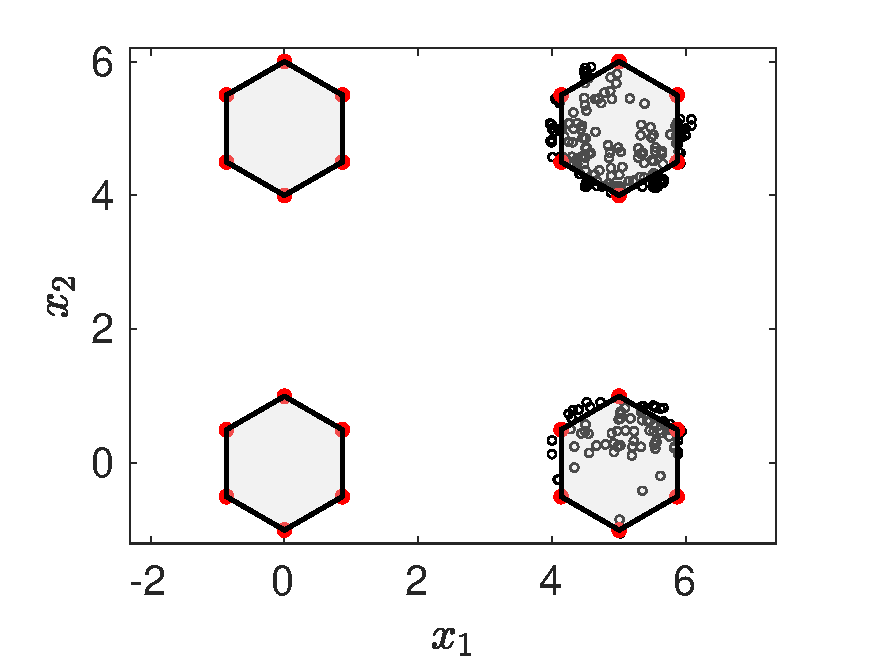
\includegraphics[width=\linewidth]{Section5/dim4/PS/NSGAII}
    \caption{NSGA-II}
    \end{subfigure}
    \begin{subfigure}[b]{.24\textwidth}
    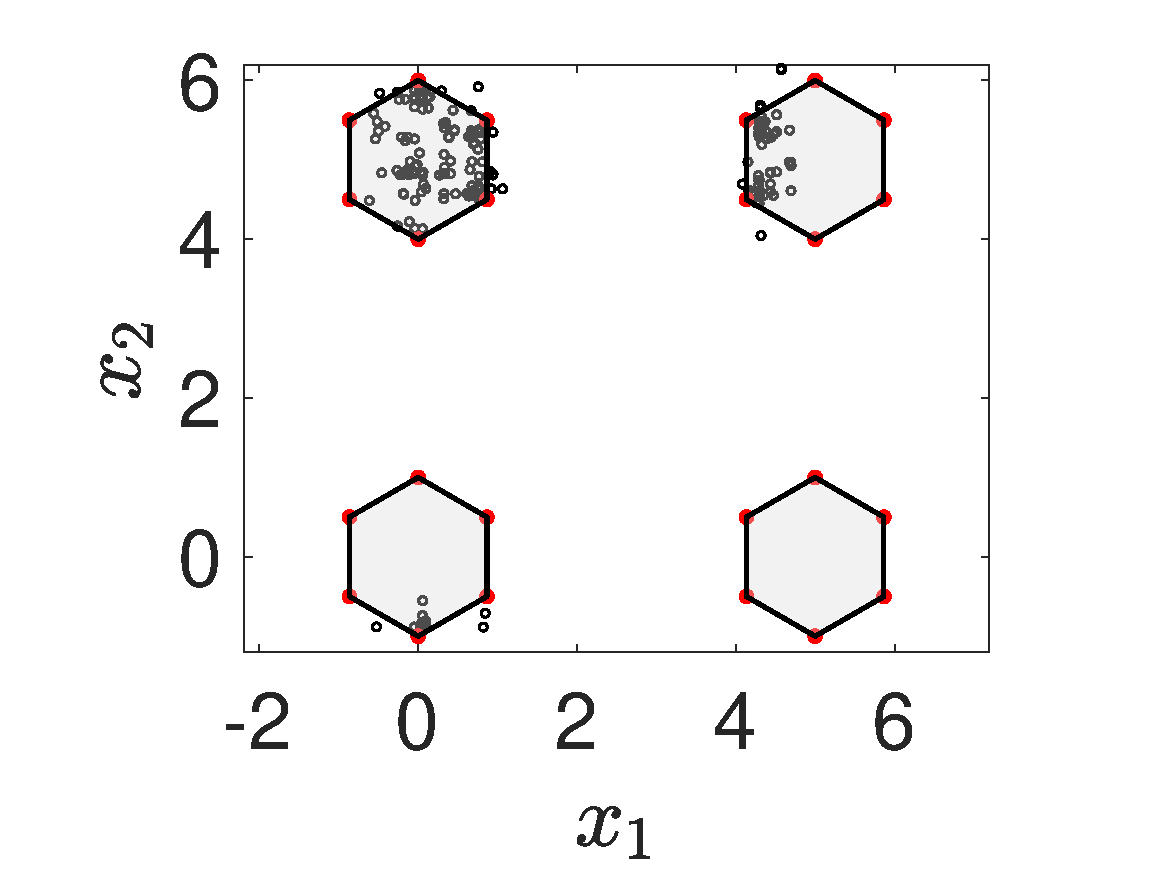
\includegraphics[width=\linewidth]{Section5/dim4/PS/NSGAIII}
    \caption{NSGA-III}
    \end{subfigure}
    
    \begin{subfigure}[b]{.24\textwidth}
    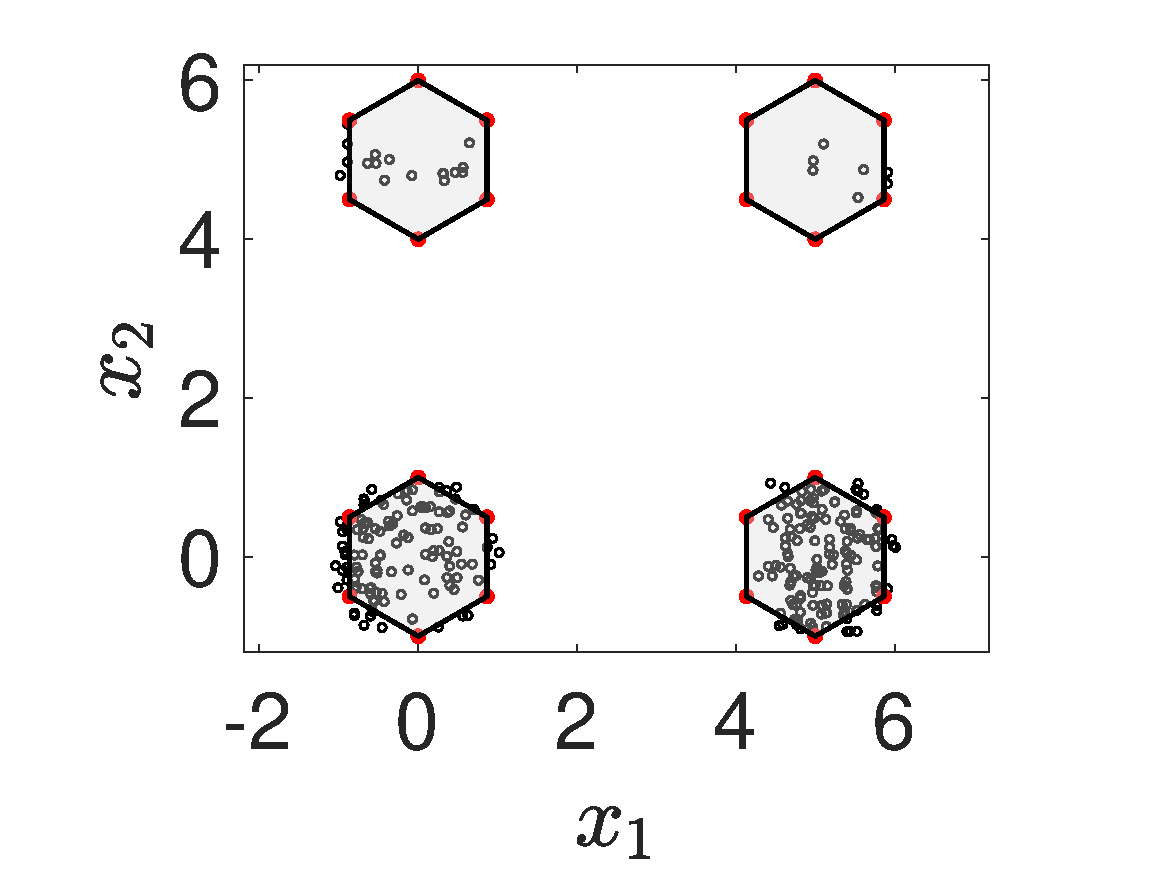
\includegraphics[width=\linewidth]{Section5/dim4/PS/SPEA2}
    \caption{SPEA2}
    \end{subfigure}
    \begin{subfigure}[b]{.24\textwidth}
    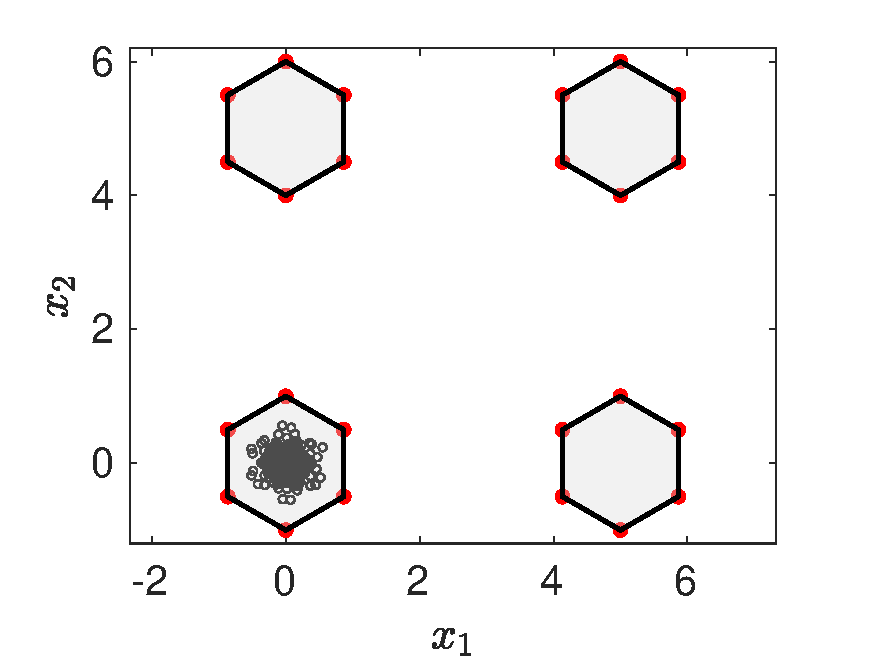
\includegraphics[width=\linewidth]{Section5/dim4/PS/MOEAD_TCH}
    \caption{MOEA/D-TCH}
    \end{subfigure}
    
    \begin{subfigure}[b]{.24\textwidth}
    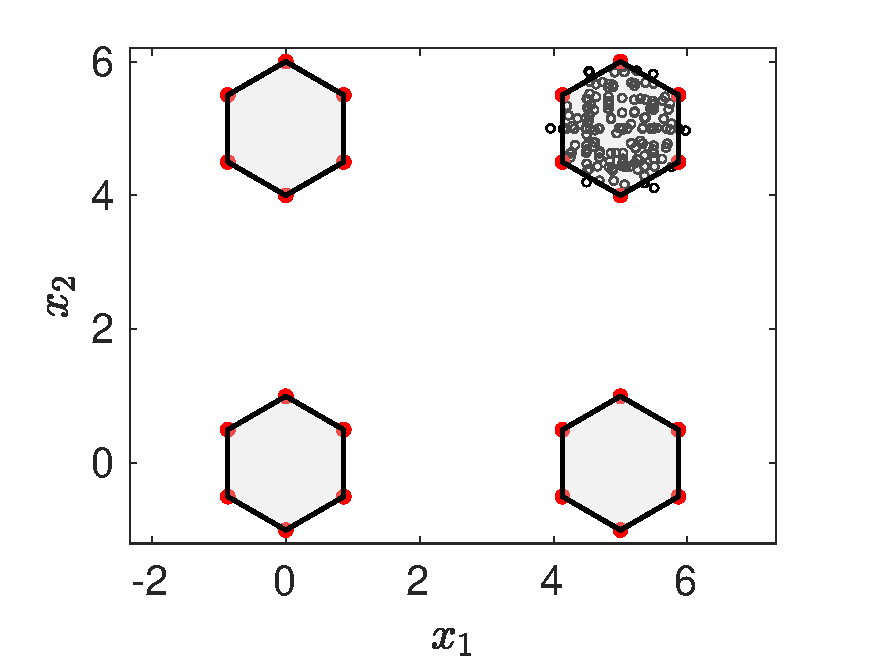
\includegraphics[width=\linewidth]{Section5/dim4/PS/MOEAD_PBI}
    \caption{MOEA/D-PBI}
    \end{subfigure}
    \begin{subfigure}[b]{.24\textwidth}
    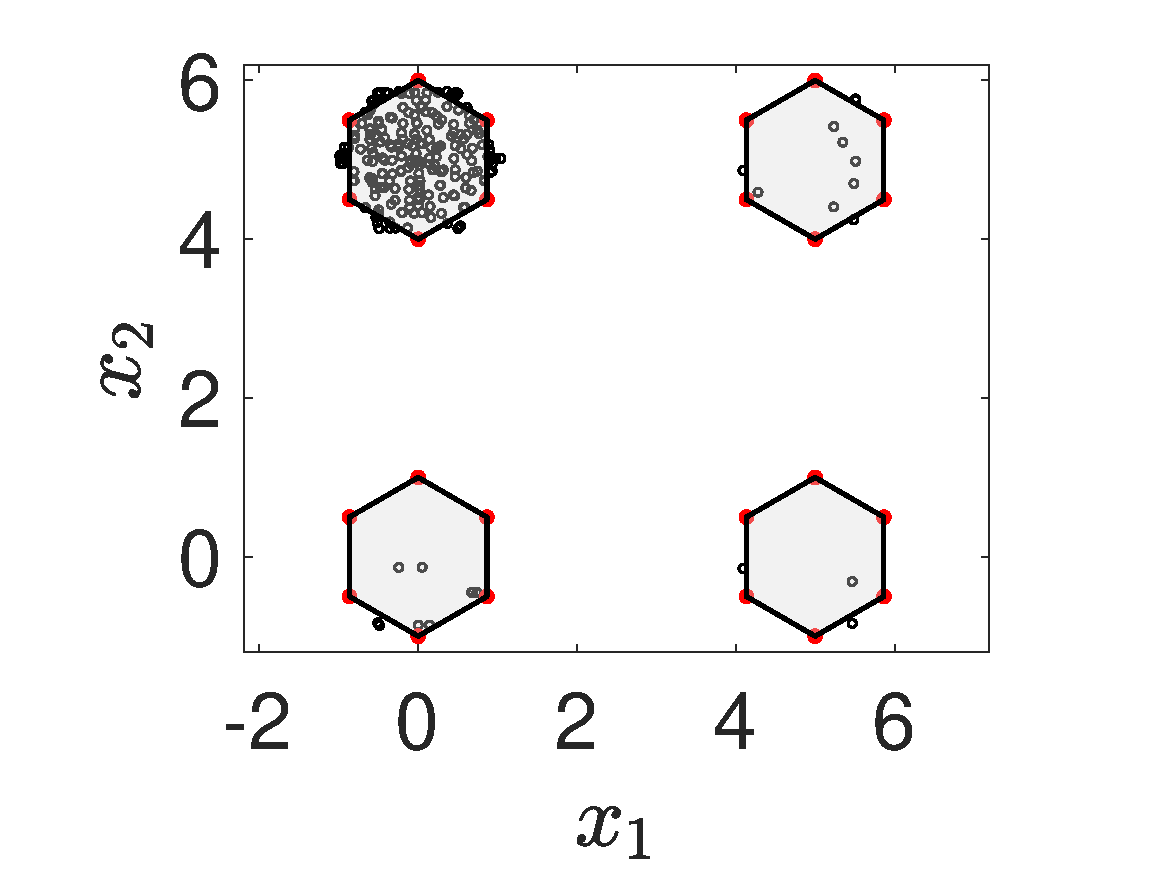
\includegraphics[width=\linewidth]{Section5/dim4/PS/IBEA}
    \caption{IBEA}
    \end{subfigure}

    \caption{Simulation results of MOEAs on multi-polygon test problem with $D=4$.}
    \label{fig: MOEAs PS dim=4}
\end{figure}

\begin{figure}[t!]
    \centering
    \begin{subfigure}[b]{.24\textwidth}
    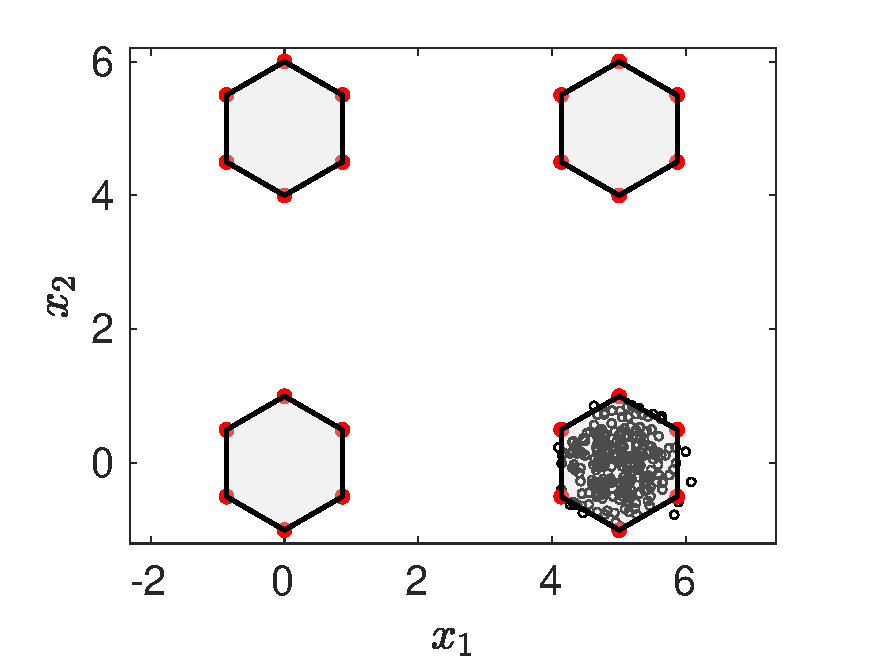
\includegraphics[width=\linewidth]{Section5/dim4/PS/DNEA}
    \caption{DNEA}
    \end{subfigure}
    \begin{subfigure}[b]{.24\textwidth}
    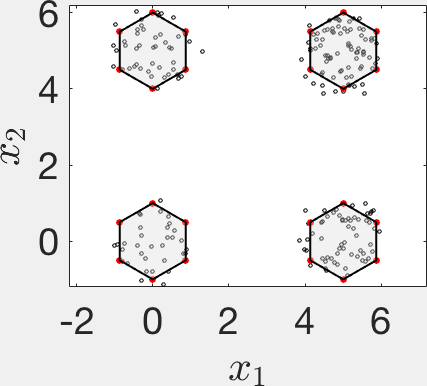
\includegraphics[width=\linewidth]{Section5/dim4/PS/MO_Ring_PSO_SCD}
    \caption{MO\_Ring\_PSO\_SCD}
    \end{subfigure}
    
    \begin{subfigure}[b]{.24\textwidth}
    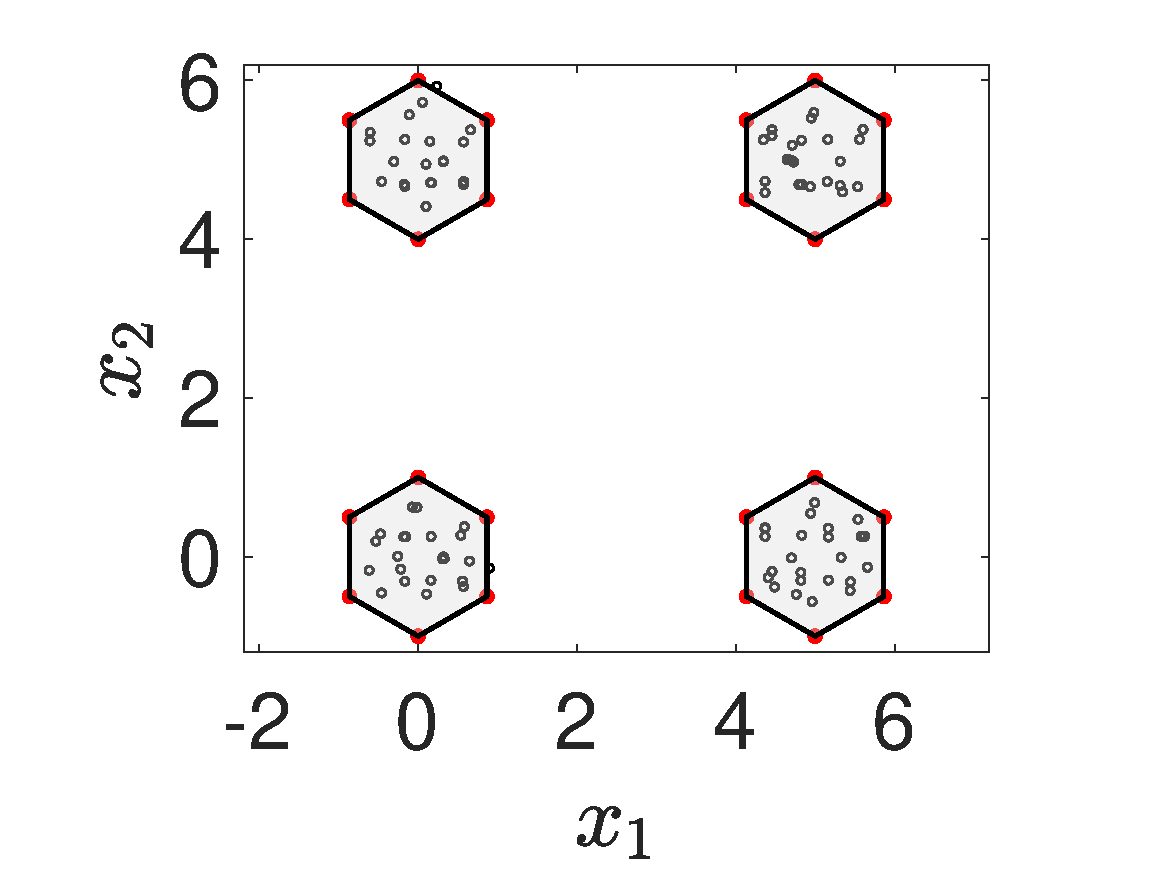
\includegraphics[width=\linewidth]{Section5/dim4/PS/MOEADAD}
    \caption{MOEA/D-AD}
    \end{subfigure}
    \begin{subfigure}[b]{.24\textwidth}
    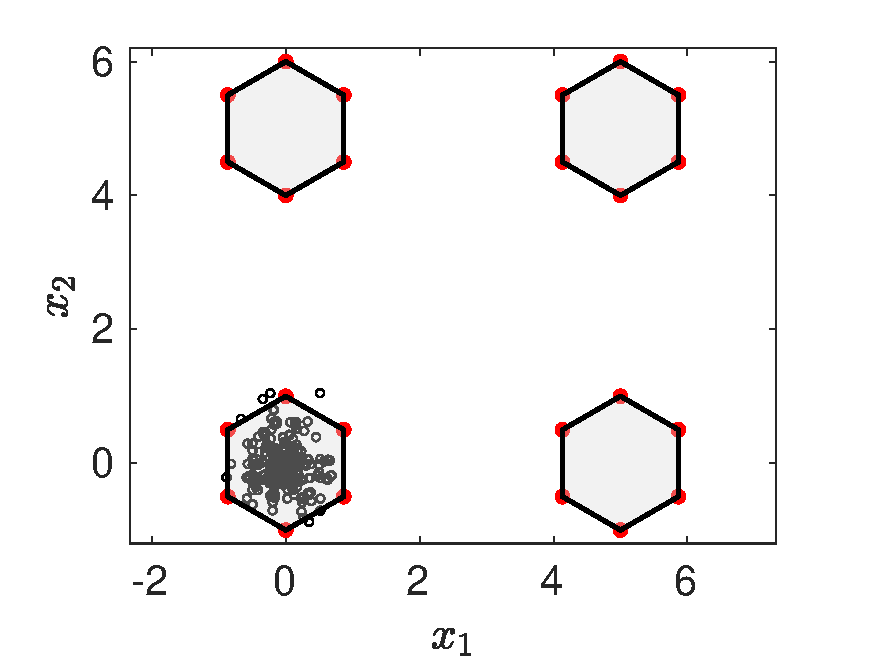
\includegraphics[width=\linewidth]{Section5/dim4/PS/OmniOptimizer}
    \caption{Omni-optimizer}
    \end{subfigure}
    \caption{Simulation results of MMEAs on multi-polygon test problem with $D=4$.}
    \label{fig: MMEAs PS dim=4}
\end{figure}

We also examine the number of solutions in each area (areas 1 \textasciitilde 4) during the evolution. From Figs. \ref{fig: MOEAs Diversity dim=4} and \ref{fig: MMEAs Diversity dim=4}, we can see that the slight increase in the number of decision variables from two to four makes it very difficult to maintain the diversity of solutions over the four polygons. In Fig. \ref{fig: MMEAs Diversity dim=4}, the diversity of the population in the decision space of DNEA and Omni-optimizer quickly disappears. These two MMEAs failed to obtain a good solution set that covers all polygons when $D=4$. 

%% dim = 4 Diversity Plot
\begin{figure}[t!]
    \centering
    \begin{subfigure}[b]{.24\textwidth}
    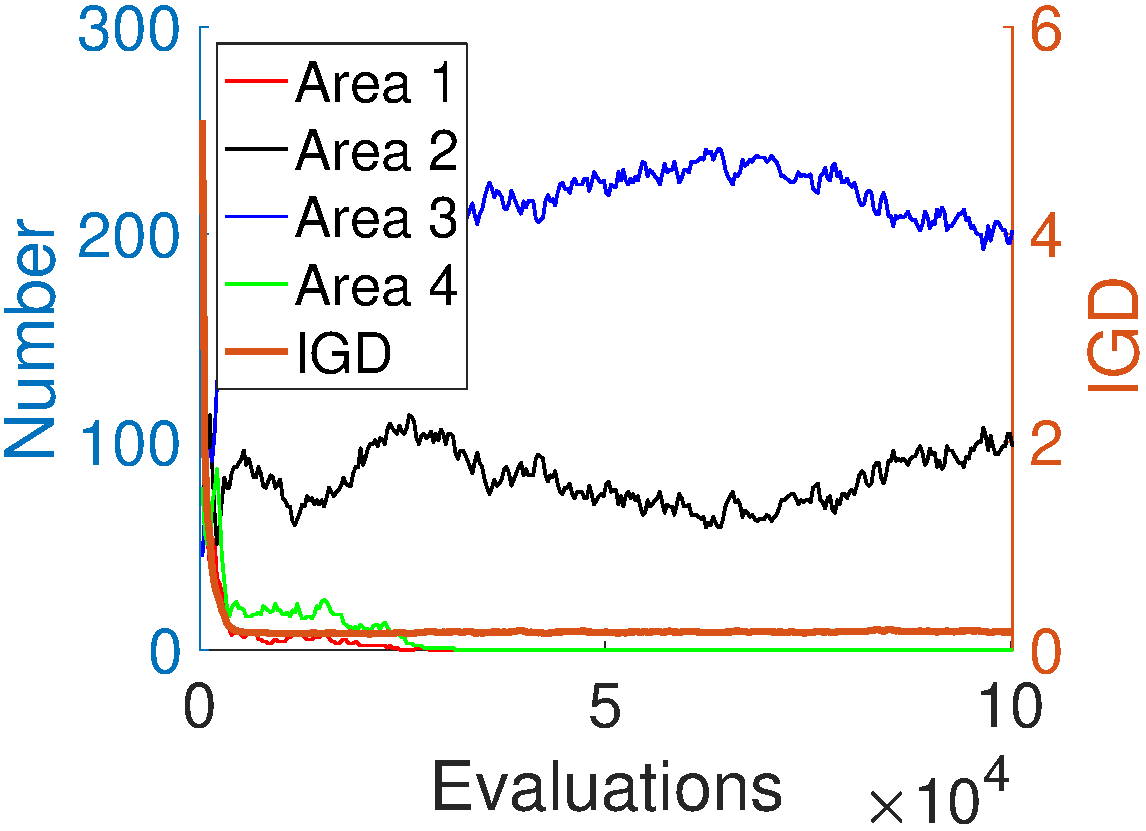
\includegraphics[width=\linewidth]{Section5/dim4/Diversity/NSGAII}
    \caption{NSGA-II}
    \end{subfigure}
    \begin{subfigure}[b]{.24\textwidth}
    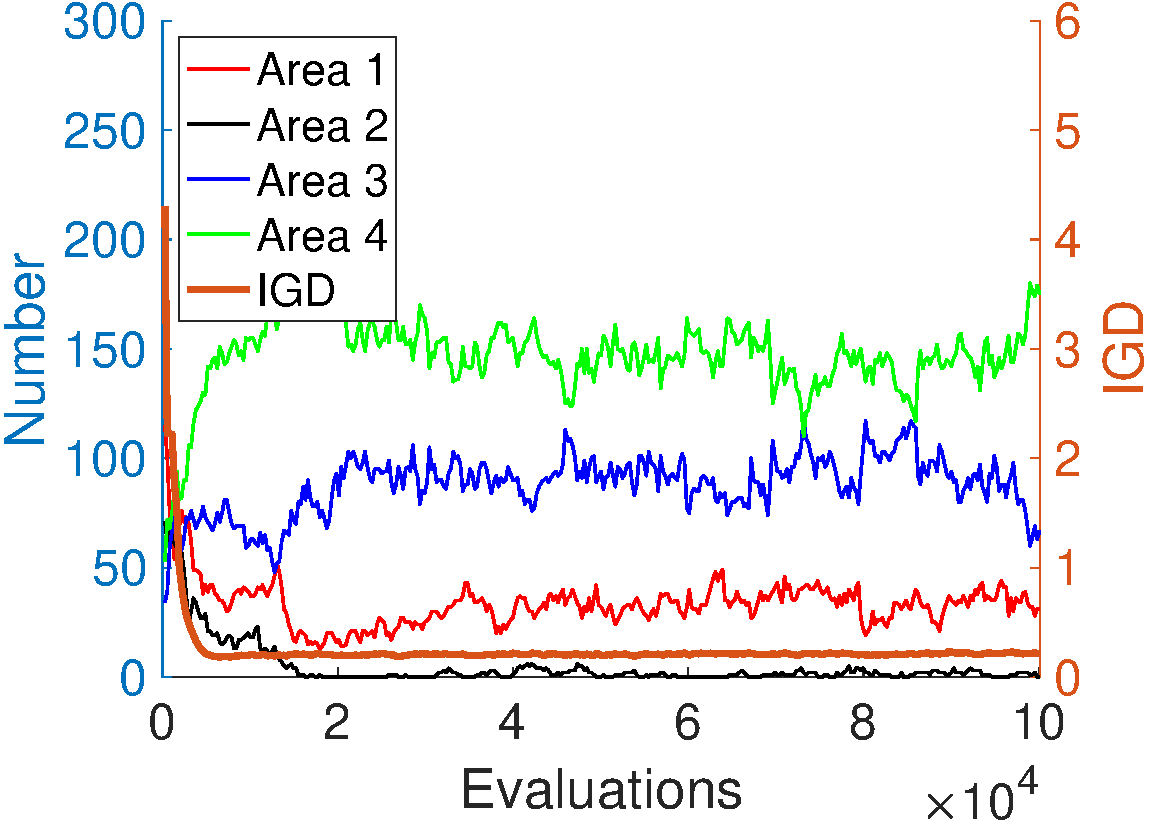
\includegraphics[width=\linewidth]{Section5/dim4/Diversity/NSGAIII}
    \caption{NSGA-III}
    \end{subfigure}
    
    \begin{subfigure}[b]{.24\textwidth}
    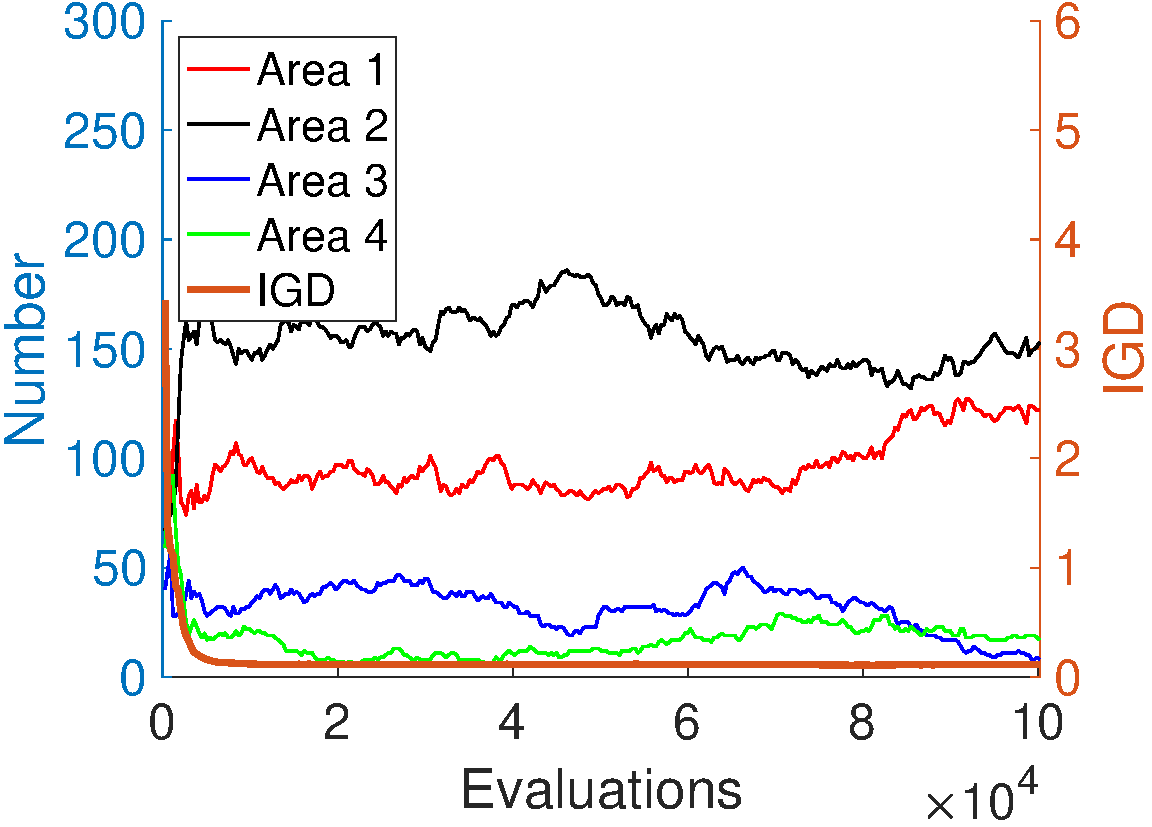
\includegraphics[width=\linewidth]{Section5/dim4/Diversity/SPEA2}
    \caption{SPEA2}
    \end{subfigure}
    \begin{subfigure}[b]{.24\textwidth}
    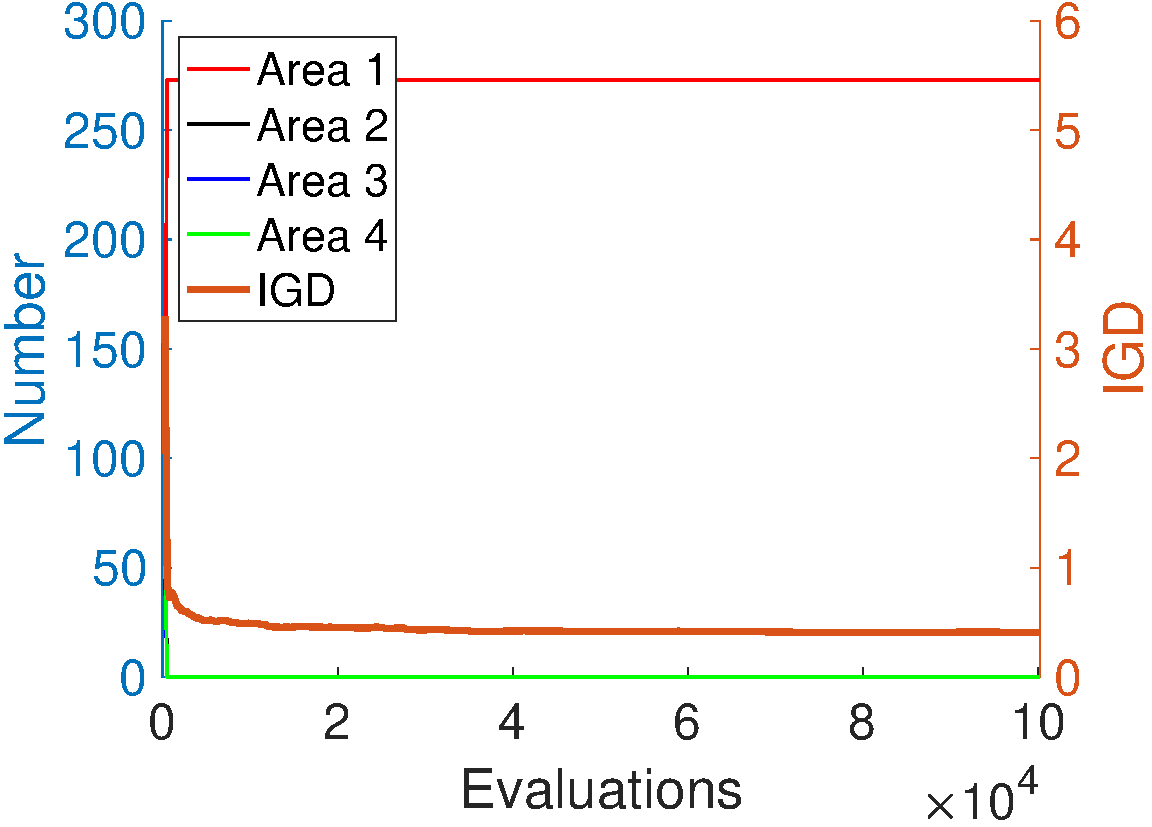
\includegraphics[width=\linewidth]{Section5/dim4/Diversity/MOEAD_TCH}
    \caption{MOEA/D-TCH}
    
    \end{subfigure}
    \begin{subfigure}[b]{.24\textwidth}
    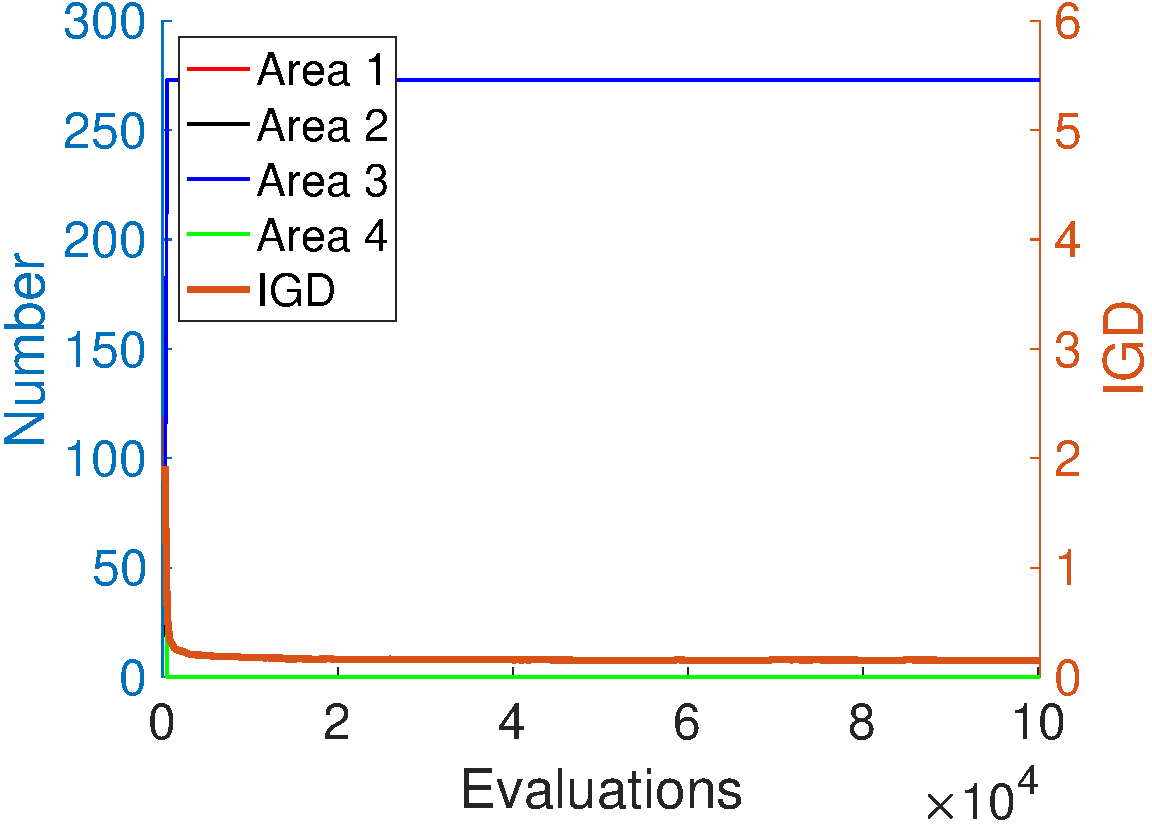
\includegraphics[width=\linewidth]{Section5/dim4/Diversity/MOEAD_PBI}
    \caption{MOEA/D-PBI}
    \end{subfigure}
    \begin{subfigure}[b]{.24\textwidth}
    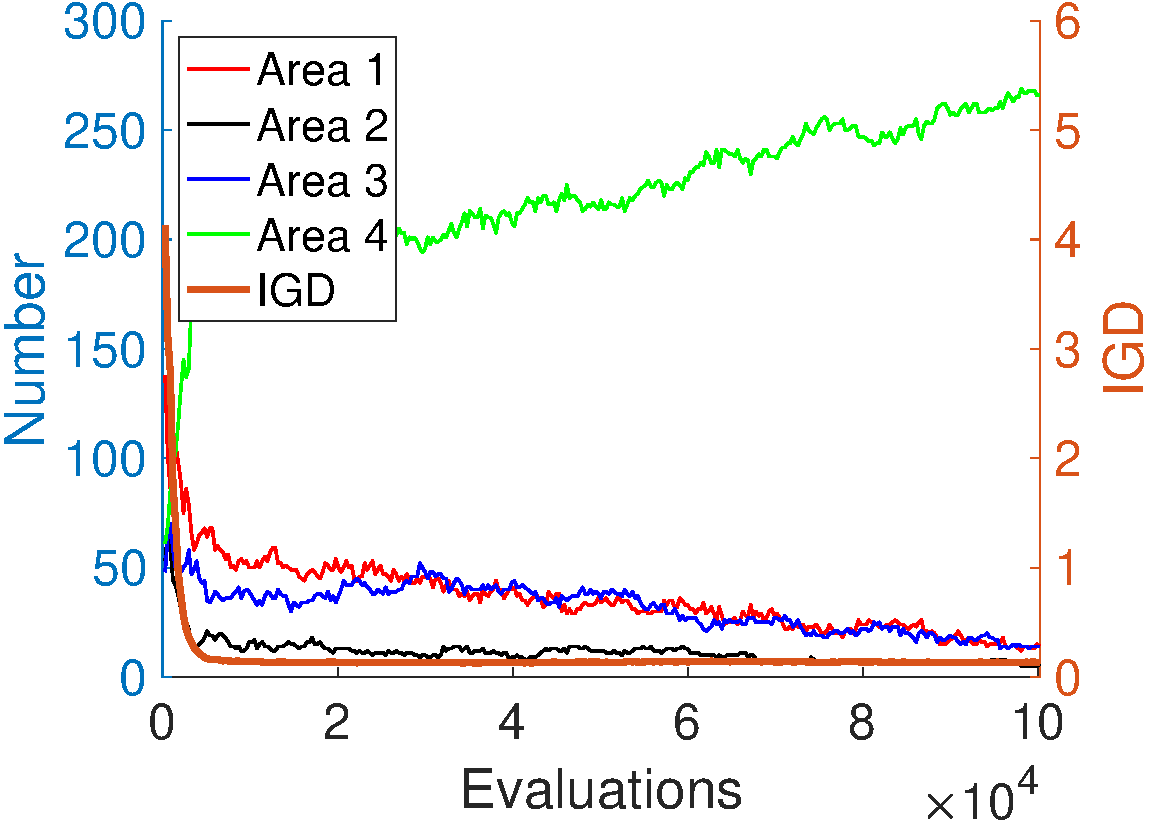
\includegraphics[width=\linewidth]{Section5/dim4/Diversity/IBEA}
    \caption{IBEA}
    \end{subfigure}

    \caption{The number of solutions in each area and the IGD value through the evolution by each MOEA on the multi-polygon test problem with $D=4$.}
    \label{fig: MOEAs Diversity dim=4}
\end{figure}

\begin{figure}[t!]
    \centering
    \begin{subfigure}[b]{.24\textwidth}
    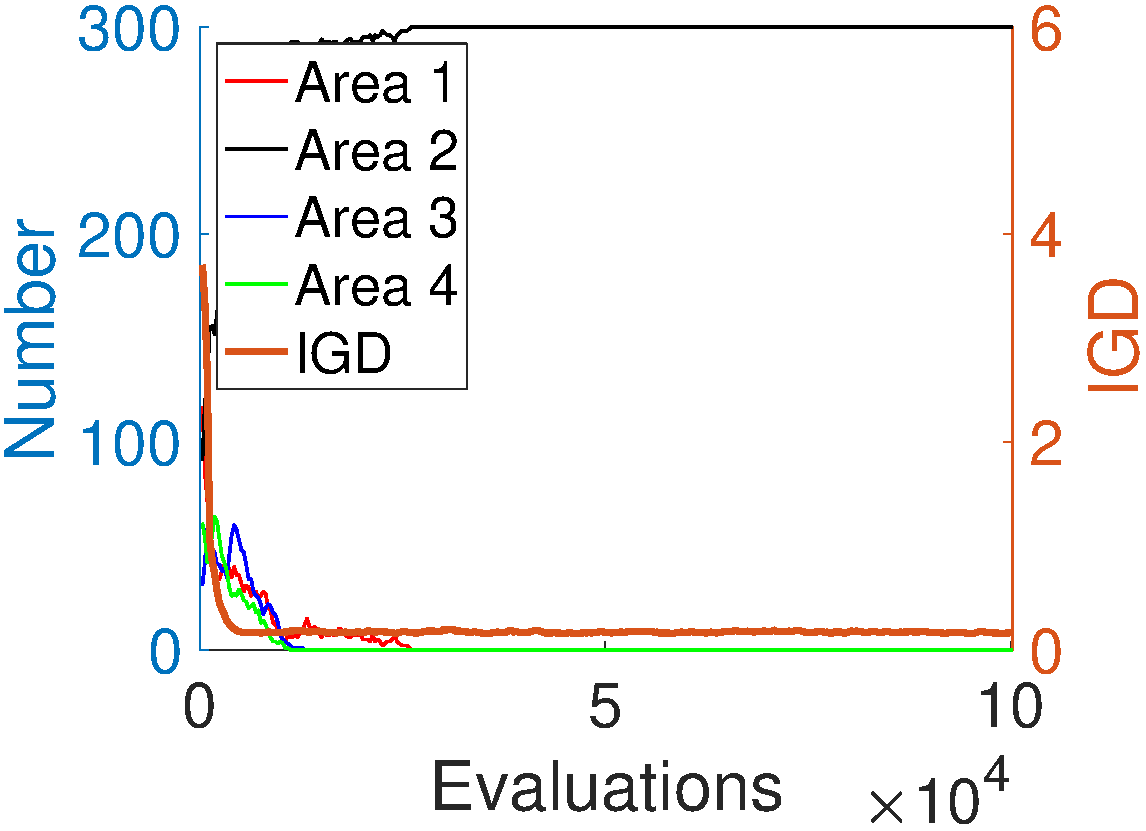
\includegraphics[width=\linewidth]{Section5/dim4/Diversity/DNEA}
    \caption{DNEA}
    \end{subfigure}
    \begin{subfigure}[b]{.24\textwidth}
    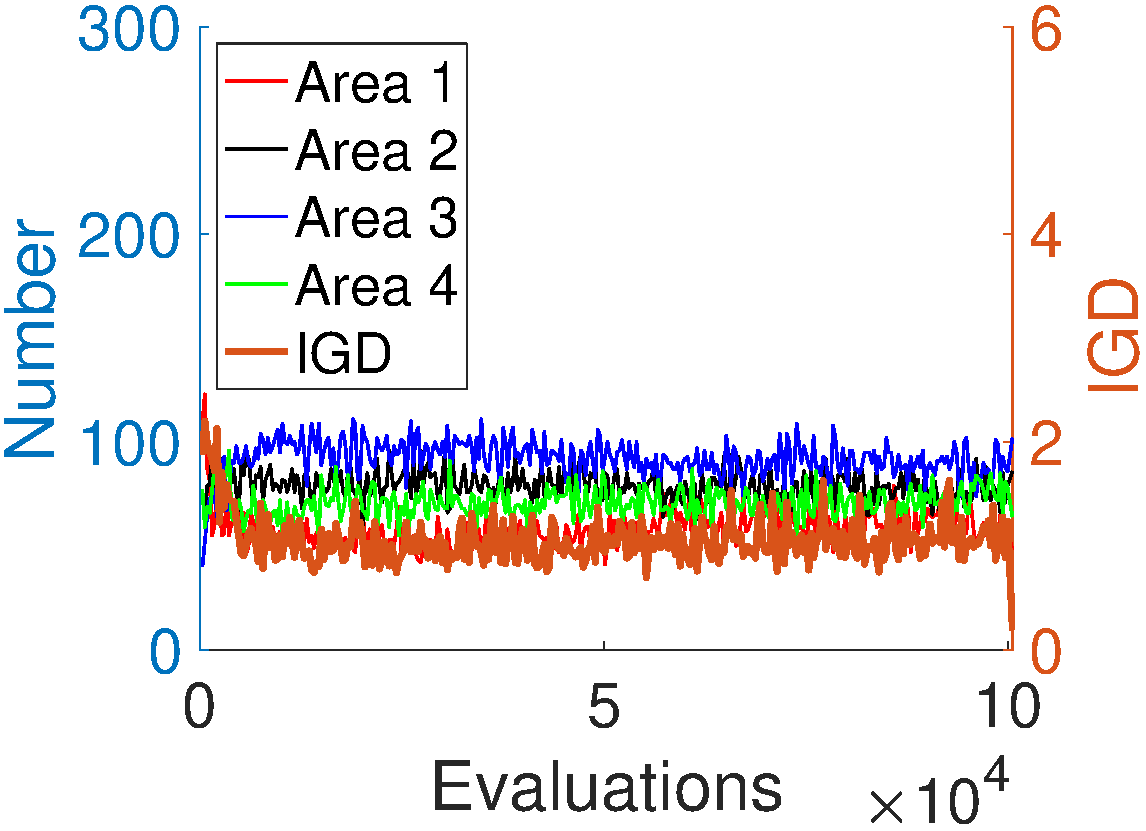
\includegraphics[width=\linewidth]{Section5/dim4/Diversity/MO_Ring_PSO_SCD}
    \caption{MO\_Ring\_PSO\_SCD}
    \end{subfigure}
    
    \begin{subfigure}[b]{.24\textwidth}
    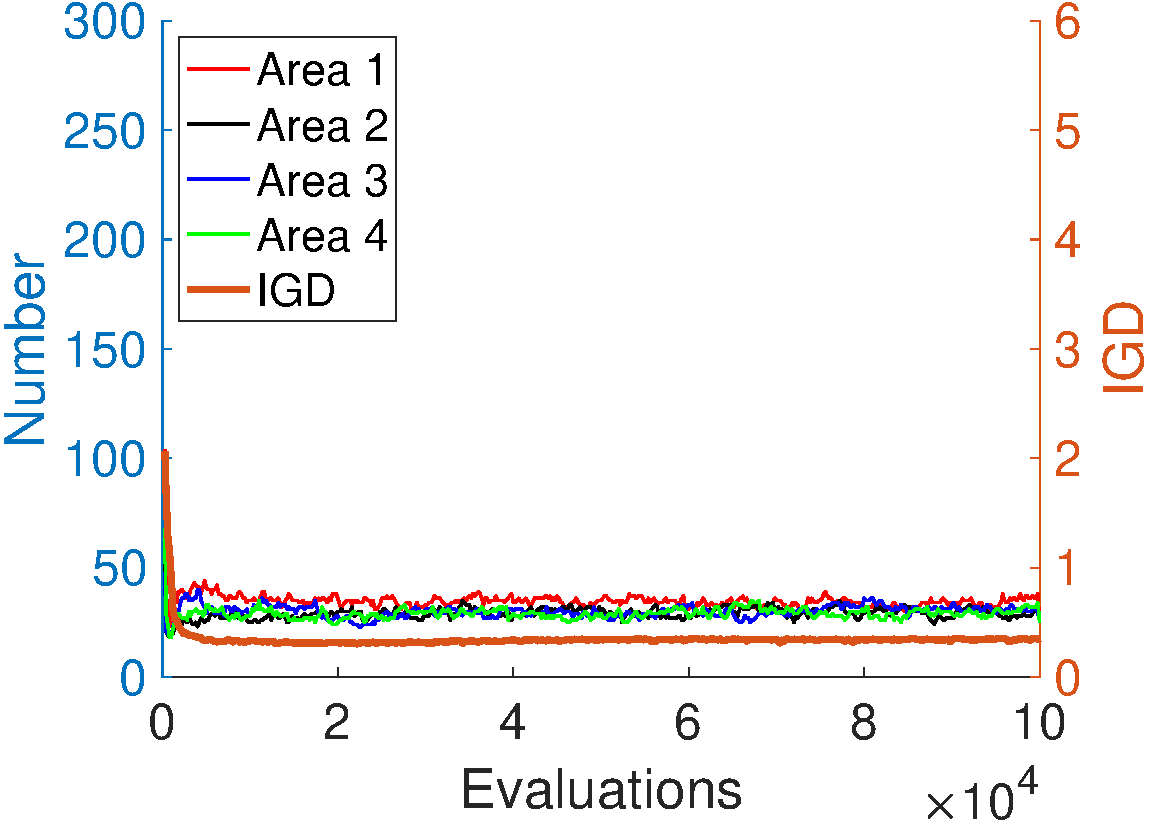
\includegraphics[width=\linewidth]{Section5/dim4/Diversity/MOEADAD}
    \caption{MOEA/D-AD}
    \end{subfigure}
    \begin{subfigure}[b]{.24\textwidth}
    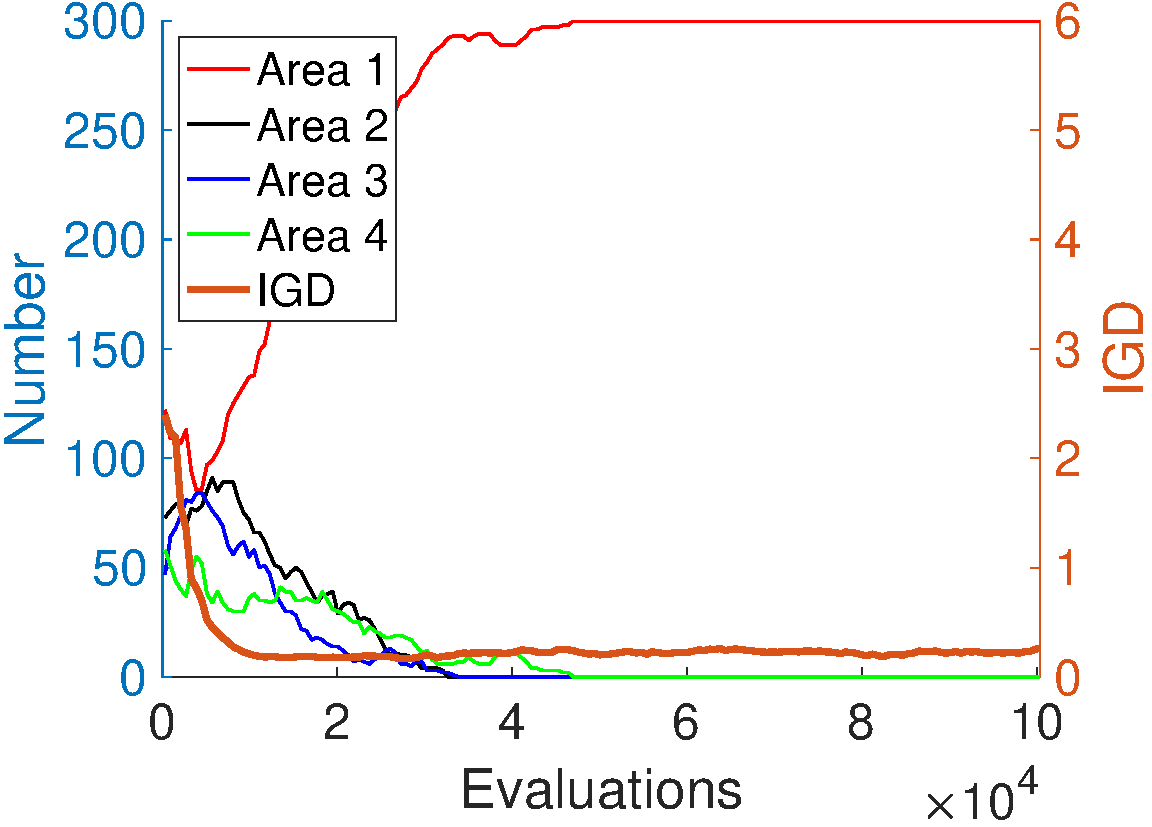
\includegraphics[width=\linewidth]{Section5/dim4/Diversity/OmniOptimizer}
    \caption{Omni-optimizer}
    \end{subfigure}
    \caption{The number of solutions in each area and the IGD value through the evolution by each MMEA on the multi-polygon test problem with $D=4$.}
    \label{fig: MMEAs Diversity dim=4}
\end{figure}

Due to the page limitation, the simulation results of MOEAs and MMEAs on multi-polygons test problem with 6, 8, 10 and 100 decision variables are not shown here. Instead, we show the IGDX\cite{liang2016multimodal} and IGD values of each algorithm when $D=2, 4, 6, 8, 10, 100$ in Table \ref{table: IGDX sumup} and \ref{table: IGD sumup}, respectively. These values are calculated for the representative single run. The IGD and IGDX indicators measure the quality of the solution set in the objective and decision space, respectively. In each table, the best values in each column (i.e, for each test problem) are highlighted in yellow. In Table \ref{table: IGDX sumup}, clearly better results (i.e, clearly smaller IGDX values) are obtained by MO\_Ring\_PSO\_SCD and MOEA/D-AD than other algorithms for the test problems with $D = 4, 6, 8, 10$, this observation is consistent with our visualization results in Figs. \ref{fig: MOEAs PS dim=4} and \ref{fig: MMEAs PS dim=4}.

\begin{table}[t!]
\centering
\caption{IGDX Values}
\begin{tabular}{@{}ccccccc@{}}
\toprule
Algorithms      & D=2                          & D=4                          & D=6                          & D=8                          & D=10                         & D=100                         \\ \midrule
NSGA-II         & 0.14                         & 2.71                         & 4.81                         & 6.67                         & 8.09                         & 28.44                         \\
NSGA-III        & 1.53                         & 3.4                          & 5.2                          & 6.87                         & 8.15                         & 29.56                         \\
SPEA2           & \cellcolor[HTML]{F8FF00}0.11 & 1.84                         & 4.74                         & 6.87                         & 7.85                         & \cellcolor[HTML]{F8FF00}28.45 \\
MOEA/D-TCH      & 1.17                         & 5.53                         & 6.91                         & 8.13                         & 9.22                          & 31.06                         \\
MOEA/D-PBI      & 1.96                         & 4.96                         & 6.29                         & 7.32                         & 8.26                         & 29.73                         \\
IBEA            & 0.13                         & 1.8                          & 5.03                         & 6.91                         & 7.82                         & 29.52                         \\
DNEA            & 0.12                         & 5.13                         & 6.49                         & 7.69                         & 8.73                         & 30.74                         \\
MO\_Ring\_PSO\_SCD & \cellcolor[HTML]{F8FF00}0.11 & 0.33                         & 0.68                         & 1.13                         & 1.9                          & 44.08                         \\
MOEA/D-AD       & 0.19                         & \cellcolor[HTML]{F8FF00}0.28 & \cellcolor[HTML]{F8FF00}0.41 & \cellcolor[HTML]{F8FF00}0.57 & \cellcolor[HTML]{F8FF00}0.82 & 32.96                         \\
Omni-optimizer  & 0.16                         & 5.08                         & 6.47                         & 7.83                         & 9.02                         & 30.62                         \\ \bottomrule
\end{tabular}
\label{table: IGDX sumup}
\end{table}

 However, in Table \ref{table: IGD sumup}, the IGD values of MMEAs are usually larger than MOEAs especially when $D$ is large. IBEA and SPEA2 outperform other algorithms in terms of the quality of solutions in the objective space. This observation has been reported in \cite{liang2016multimodal}, \cite{tanabe2018decomposition} and \cite{shir2009enhancing}. 
 
 Weaker performance of MMEAs than MOEAs in the objective space can be interpreted below. Suppose an MMOP has $K$ equivalent Pareto sets and the population size in an MMEA in $N$. Ideally, the MMEA uses $1/K$ of $N$ individuals to locate each Pareto set. This MMEA is similar to an MOEA with population size = $N/K$. Smaller population size usually means weaker search power. Another reason is that diversification mechanisms of MMEAs in the decision space do not improve the distribution of solutions in the objective space (i.e. do not improve the IGD value). On the contrary, diversification mechanisms of MOEAs focus on the distribution of solutions in the objective space, which usually improve the IGD value. 
 
 In Table \ref{table: Perpendicular Distance}, we show the average perpendicular distances of solutions in the final population to the target plane for each algorithm. In the case of $D=2$, the perpendicular distance of all solutions are always zeros since all solutions are on the two-dimensional plane. The average perpendicular distance is an index of the convergence of solutions in the $D$-dimensional decision space to the hyper-plane with the polygons. It is clear from Table \ref{table: Perpendicular Distance} that  MMEAs (MOEA/D-AD and MO\_Ring\_PSO\_SCD) have weaker convergence ability than most of the other algorithms. Especially, in the case of $D=100$, these two algorithms clearly shows the weakest convergence ability among all the examined algorithms in Table \ref{table: Perpendicular Distance}. As a result, these two algorithms are also the worst in Table \ref{table: IGD sumup} with respect to IGD in the case of $D = 100$. In Table \ref{table: IGDX sumup}, all algorithms show similar performance with respect to IGDX in the case of $D=100$ (i.e., no algorithm works well on the test problem with $D=100$). The main reason for the poor performance of MOEA/D-AD and MO\_Ring\_PSO\_SCD may be weak diversification mechanisms for the other algorithms.

\begin{table}[t!]
\centering
\caption{IGD Values}
\begin{tabular}{@{}ccccccc@{}}
\toprule
Algorithms      & D=2                          & D=4                          & D=6                          & D=8                          & D=10                        & D=100                        \\ \midrule
NSGA-II         & 0.1                          & 0.17                         & 0.25                         & 0.33                         & 0.41                        & 3.01                         \\
NSGA-III        & 0.14                         & 0.21                         & 0.28                         & 0.33                         & 0.39                        & 3.95                         \\
SPEA2           & \cellcolor[HTML]{F8FF00}0.07 & \cellcolor[HTML]{F8FF00}0.12 & 0.16                         & 0.2                          & 0.24                        & \cellcolor[HTML]{F8FF00}2.73 \\
MOEA/D-TCH      & 0.26                         & 0.41                         & 0.64                         & 0.93                         & 1.2                         & 6.76                         \\
MOEA/D-PBI      & 0.11                         & 0.16                         & 0.2                          & 0.25                         & 0.3                         & 4.22                          \\
IBEA            & 0.09                         & 0.13                         & \cellcolor[HTML]{F8FF00}0.15 & \cellcolor[HTML]{F8FF00}0.17 & \cellcolor[HTML]{F8FF00}0.2 & 3.9                          \\
DNEA            & 0.08                         & 0.17                         & 0.31                         & 0.5                          & 0.67                        & 5.91                         \\
MO\_Ring\_PSO\_SCD & 0.1                          & 0.19                         & 0.4                          & 0.72                         & 1.12                        & 57.46                        \\
MOEA/D-AD       & 0.27                         & 0.36                         & 0.47                         & 0.58                         & 0.72                        & 12.97                        \\
Omni-optimizer  & 0.09                         & 0.22                          & 0.45                         & 0.7                          & 0.95                        & 5.54                         \\ \bottomrule
\end{tabular}
\label{table: IGD sumup}
\end{table}

\begin{table}[t!]
\centering
\caption{Average Perpendicular Distances}
\begin{tabular}{@{}ccccccc@{}}
\toprule
Algorithms         & D=2 & D=4                           & D=6                           & D=8                           & D=10                          & D=100                         \\ \midrule
NSGA-II            & 0  & 0.18                         & 0.31                         & 0.41                         & 0.57                         & 3.85                         \\
NSGA-III           & 0  & 0.18                         & 0.31                         & 0.39                         & 0.48                         & 2.77                         \\
SPEA2              & 0  & 0.18                         & 0.3                          & 0.41                         & 0.49                         & 2.98                         \\
MOEA/D-TCH         & 0  & \cellcolor[HTML]{F8FF00}0.01 & \cellcolor[HTML]{F8FF00}0.05 & \cellcolor[HTML]{F8FF00}0.05 & \cellcolor[HTML]{F8FF00}0.07 & \cellcolor[HTML]{F8FF00}0.31 \\
MOEA/D-PBI         & 0  & 0.08                         & 0.16                         & 0.25                         & 0.3                          & 1.53                         \\
IBEA               & 0  & 0.03                         & 0.06                         & 0.12                         & 0.18                         & 1.61                         \\
DNEA               & 0  & 0.23                         & 0.36                         & 0.43                         & 0.5                          & 1.37                         \\
MO\_Ring\_PSO\_SCD & 0  & 0.28                         & 0.66                         & 1.05                         & 1.43                         & 32.01                        \\
MOEA/D-AD          & 0  & 0.09                         & 0.18                         & 0.31                         & 0.48                         & 10.26                        \\
Omni-optimizer     & 0  & 0.22                      & 0.31                         & 0.4                          & 0.41                         & 2.68                         \\ \bottomrule
\end{tabular}
\label{table: Perpendicular Distance}
\end{table}
\section{Conclusion}
\label{Conclusion}
In this paper, we first addressed the difficulties in solving MMOPs in detail. We pointed out that the selection, mutation and crossover operators in standard MOEAs are likely to decrease the diversity of solutions in the decision space when handling MMOPs. Using the concept of genetic drift, we explained the decrease in the diversity of solutions in the decision space when MOEAs are applied to MMOPs. The experimental results showed that two MMEAs MO\_Ring\_PSO\_SCD and MOEA/D-AD have best performance than DNEA, Omni-optimizer and the examined MOEAs in terms of preserving the diversity in the decision space. However, our experimental results also shows that these two high-performance MMEAs have weaker convergence ability than the other examined algorithms (both MMEAs and MOEAs). These observations clearly suggest the difficulty in simultaneously realizing high convergence ability and high diversification ability.

Further computation experiments on various MMOPs are needed to examine the problem-dependency of the performance of each MMEA. In this paper, we mainly focuses on the scalability of each algorithm with respect to the number of decision variables. We need to examine other aspects of the scalability such as the number of objectives and the number of equivalent Pareto sets. Multi-polygon problems in high-dimensional decision spaces can be used to examine various aspects of the scalability. Of course, our final goal is to design a high-performance MMEA with respect to both the convergence ability and the diversification ability.
\section*{Acknowledgement}
This work was supported by National Natural Science Foundation of China (Grant No. 61876075), the Program for Guangdong Introducing Innovative and Enterpreneurial Teams (Grant No. 2017ZT07X386), Shenzhen Peacock Plan (Grant No. KQTD2016112514355531), the Science and Technology Innovation Committee Foundation of Shenzhen (Grant No. ZDSYS201703031748284), and the Program for University Key Laboratory of Guangdong Province (Grant No. 2017KSYS008).
\bibliographystyle{ieeetr}
\bibliography{Reference.bib}

\end{document}
